\documentclass[11pt]{article}
\usepackage{hyperref}
\usepackage{amsmath}
\usepackage{amsfonts}

\usepackage{graphicx}
\usepackage{lscape}
\usepackage[nolists,tablesfirst,nomarkers]{endfloat}
\usepackage{setspace}


\setlength{\textwidth}{6.5in} \setlength{\textheight}{8.8in}
\setlength{\topmargin}{-0.40in} \setlength{\oddsidemargin}{0in}
\setlength{\parskip}{3mm}

\IfFileExists{pslatex.sty}{
\usepackage{pslatex}
}{}


\begin{document}

\title{\textbf{Data file explanation}}

\newpage \renewcommand{\thefootnote}{\arabic{footnote}}
\setcounter{page}{1}


{\bf \large Data files:}
\begin{enumerate}
\item {\bf	Liborswapdata.csv}

Format: date(excelserial number), (1,2,3,6,9,12)-month Libor, (2,3,4,5,7,10,15,20,30)-year swap rates

Table 1 summary statistics can be directly computed from these rates. The data are sampled weekly.

\item {\bf	Model3outputs.csv}

Format: date, (x1,x2,x3)(3 factors), fitted values on the 15-libor and swap rates in the same order as the previous data

\item {\bf	Model15output.csv}

Format: date, (x1,x2,x3, $\cdots$,x15)(15 factors), fitted values on the 15-libor and swap rates in the same order as the previous data

\item {\bf	osXhat15.csv}

Format: date, (x1,x2,x3,$\cdots$,x15)


Fitted factor values $\widehat{X}_{t}$ for out of sample testing periods.

The values $\widehat{X}_t$ at each date $t$ are generated from a different set of parameter estimates. The parameters are estimated using data up to that date $t$.

\item {\bf	osXPred15h1.csv}

Format: date, (x1,x2,x3,$\cdots$,x15)

Forecasted factor values $\overline{X}_{t+h}$ for out of sample testing periods from week 158 (1998/1/7) forward, with $h=1$ week.

For ease of comparison, the file length is kept the same as the other files, but filled with NaNs for the first 157 weeks.




\item {\bf	osXPred15h2.csv}

Format: date, (x1,x2,x3,$\cdots$,x15)

Forecasted factor values $\overline{X}_{t+h}$ for out of sample testing periods, with $h=2$ weeks.


\item {\bf	osXPred15h3.csv}

Format: date, (x1,x2,x3,$\cdots$,x15)

Forecasted factor values $\overline{X}_{t+h}$ for out of sample testing periods, with $h=3$ weeks.


\item {\bf	osXPred15h4.csv}

Format: date, (x1,x2,x3,$\cdots$,x15)

Forecasted factor values $\overline{X}_{t+h}$ for out of sample testing periods, with $h=4$ week.

\item {\bf	osparameters15.csv}

Format: date, parameters



The estimated parameter values at each date $t$ using data up to that date for the 15-factor model.

Let $p$ denote the list of parameters. They correspond to the model parameters in the paper as follows:
\[
\kappa_1=e^{p_1},\quad
\sigma_r=e^{p_2},\quad
\theta^{\mathbb{Q}}_r=e^{p_3},\quad
b=e^{e^{p_4}},\quad
\theta_r=e^{p_5},\quad
\sigma_e^2=e^{p_6}
\]

\end{enumerate}

\newpage

{\bf \large Output Statistics:}

\begin{enumerate}
\item {\bf	Table 1}

Summary statistics can be directly computed from the libor and swap rates from  {\bf	Liborswapdata.csv}. 

\item {\bf	Table 3}

The pricing error statistics in Table 3 can be replicated from data in three files. The pricing errors are defined as 
Error= (rates -  fitted values)*100 (in basis points)

The rates are from {\bf	Liborswapdata.csv}. The fitted values are from {\bf	Model3outputs.csv} for the three-factor model and {\bf	Model15outputs.csv} for the 15-factor model.

The reported statistics in the paper are computed using the pricing errors from the 4th week forward. The first three observations are discarded from the statistics as they can be heavily affected by the initial state assumptions. 

\item {\bf	Table 4B and 4C}

The in-sample predictive variation in Table 4B and 4C, can be replicated from the extracted factors and the parameter estimates.

At each date $t$, the factors in the data files can be regarded as $\widehat{X_t}$. Its predicted values $h$-years ahead are computed as
\[
\overline{X}_{t+h}=A+\Phi \widehat{X_t},
\]
where $A$ and $\Phi$ are functions of the estimated model parameters and forecasting horizons:
\[
\Phi=\exp(-\kappa h),\quad A=(I-\Phi)\theta,
\]
where $\kappa$ is the mean-reversion matrix with the cascade structure, $\theta$ is a vector of the long-run mean $\theta_r$.

The forecasted values of the interest rates are directly computed based on the forecasted values of the factors $\overline{X}_{t+h}$.

\item {\bf	Table 5B}

The out-of-sample predictive variation is computed in a more complex way:
\begin{enumerate}
\item At each date $t$, we use the interest rates data up to time $t$ to re-estimate the model parameters. With the re-estimated model parameters, we run through the sample to obtain the fitted factor value at date $t$, $\widehat{X_t}$. --- The difference between $\widehat{X_t}$ here for the out-of-sample statistics  and $\widehat{X_t}$ for Table 4 in-sample statistics is that the extracted factors in the in-sample statistics are based on one-set of parameter estimates whereas for the out-of-sample statistics, the factors at each date during the out-of-sample period is based on a different set of parameter estimates. 


The fitted factors $\widehat{X_t}$ for the out-of-sample statistics for the 15-factor model are in {\bf osXhat15.csv}.
 

\item The forecasting steps are the same as for the in-sample analysis.

\end{enumerate}

For ease of replication, we have also saved the predicted factor values at the reported four horizons, $\overline{X}_{t+h}$ with $h=$1,2,3,4 weeks. They are in files {\bf osXPred15h1.csv}, {\bf osXPred15h2.csv}, {\bf osXPred15h3.csv}, {\bf osXPred15h4.csv}, respectively.

Furthermore, we have also provided the parameter estimates obtained at different dates in file {\bf osparameters15.csv}. The estimates in the last date represent the full-sample estimates.


\end{enumerate}




\end{document}

The development of \textbf{[the class of]} arbitrage-free dynamic term
structure models (DTSMs) ranks as one of the most important achievements of
modern asset pricing theory.
%This framework connects the cross-sectional relation between bonds of different maturities to the evolution of the term structure,
 \emph{\textbf{This framework connects the instantaneous interest rate dynamics to the cross-sectional relation between
bonds of different maturities and its future evolution,}}
%or This framework connects the cross-sectional relation between bonds of different maturities to the instantaneous interest-rate dynamics,
    %"term structure" means in English "maturity pattern," which is a cross-sectional relation. So the whole sentence would translate to:
    %" The framework links the term structure to the evolution of the term structure."
    %For the types of models you have in mind, the model assumption is on instantaneous interest rate dynamics (normally factor dynamics and a short rate function that links short rate to the factors).
    %the model implication is on the term structure behavior (both cross-sectional and the evolution of the term structure).
    %I don't think you are referring to HJM type models here: In those models, the specification/model assumption is indeed on the evolution of the term structure,
    %the output (model implication) is options on the term structure. So you can say: HJM links the evolution/dynamics of the term structure to the cross-sectional behavior (and evolution)
    % of option prices on the term structure. The current level/shape of the term structure is assumed to be observed/known in this setup. Thus, it is neither part
    % of the model assumption, nor part of the model output. I call it initial conditions. But these initial conditions do affect the future evolution of the term structure.
    % So your original sentence is probably a better description of hjm.
while maintaining considerable scope for variation in
\textbf{modeling} %Canadian/British English uses double "l"  in "modelling," American English uses modeling.
choices. For example\textbf{,} %added comma,
the widely-used affine specifications, first characterized by
\citeasnoun{DuffieKan:96}, allow very general factor structures to govern term
structure \textbf{behavior[dynamics]}.%As I said earlier, the implication is on both the CURRENT term structure shape, and its future evolution/dynamics.
%Actually, most people focus more on the implication on the CURRENT shape (such as the stripping implication) than on future dynamics. So a more general term "behavior" is probably more appropriate as it can both mean
%the current cross-sectional relation and its future dynamics.
\footnote{Important early contributions
in the dynamic term structure literature
include \citeasnoun{Vasicek:77}, \citeasnoun{brennanschwartz:79}, %
\citeasnoun{cir:85}, \citeasnoun{Constantinides:92}, and %
\citeasnoun{LongstaffSchwartz:92}. \citeasnoun{DuffiePanSingleton:2000} and %
\citeasnoun{DuffieFilipovicSchachermayer:2003} progressively generalize the
class of affine models. \citeasnoun{LeippoldWu:2002} introduce the quadratic
class of arbitrage-free dynamic term structure models.}  Theoretical advances
in the study of these flexible, tractable models pave\emph{\textbf{[d]}} %%Is it possible to turn it into current tense?
the way for an explosion
\textbf{of[in]} %??
empirical work, including
%exhaustive efforts to explore this class and pin down appropriate specifications in pioneering work
    \emph{\textbf{comprehensive specification analysis in seminal works}}
    %pioneering means "early, first". seminal means influential. The works you cite are not early, but very influential. Or we can simply use the work influential to be exact.
    %work"s" here is one of the few places where it become plural, referring to multiple papers.
    %"comprehensive" is more appropriate than "exhaustive" because neither paper has exhausted the possible specifications.
    %An alternative, simpler sentence can be: including comprehensive (or influential, seminal, whichever you want to stress more) specification analysis by so and so.
    such as \citeasnoun{DaiSingleton:2000} and \citeasnoun{Duffee:2002}.\footnote{%
Other notable empirical contributions include
\citeasnoun{BalduzziDasForesiSundaram:96}, \citeasnoun{DaiSingleton:2002}, and
\citeasnoun{BackusForesiMozumdarWu:2001}.}

Despite these efforts, a large subset of DTSMs remains relatively unexplored. %This means the above analyses are not exhaustive:)
In particular, high-dimensional models --- \textbf{[meaning roughly]} those
having a \emph{\textbf{much}} %not sure whether we need to add a much to stress "higher". There are 4-6 factor models in the literature.
larger number of factors than the traditional three --- are more difficult to
investigate empirically because of the well-known ``curse of dimensionality.''
For example\textbf{,} %Now I see a pattern:) American English almost always have a comma after "For example, For instance, etc.
 a generic  \textbf{three-factor affine} %affine three-factor
 DTSM calls for more than twenty
parameters, and \emph{\textbf{the number of parameters [specification requirements]}} %not sure its meaning. Do you also want to imply about the efforts to perform specification analysis? not just number of parameters?
 grows rapidly with the size of the state space. \textbf{As a result,} %Therefore is fine, too. But putting is in the front separates it from the other adverb "generally" and makes the sentence flow better.
high-dimensional models are \textbf{[therefore]} generally difficult to
identify and estimate.\footnote{\emph{\textbf{See
\citeasnoun{DuffeeStanton:2007} and \citeasnoun{Duffee:2009} for recent
discussions on identification issues. Recently, in an attempt to mitigate the
identification issue, \citeasnoun{JoslinSingletonZhu:2010} provide a
normalization that
permits convenient two-step estimation of general affine models.}}} %moved up from earlier

%\footnote{Ease of implementation has not historically been a hallmark of
%empirical research on DTSMs. For recent discussion of the issues commonly
%faced, see \citeasnoun{DuffeeStanton:2007} and \citeasnoun{Duffee:2009}. Of
%particular importance is the need to carry out a highly nonlinear optimization
%over a large parameter space that in many cases is poorly identified. Recently,
%\citeasnoun{JoslinSingletonZhu:2010} (``JSZ,'' 2010) provide a normalization
%that permits convenient two-step estimation of general affine models. Their
%approach concentrates out of the likelihood parameters that can be isolated in
%the mean and autoregressive dynamics of observable factors under the objective
%density. The method offers the greatest computational benefit when there are no
%restrictions on risk premia or objective-density factor dynamics, since in this
%case the mean and autoregressive parameters under the risk-neutral and
%objective densities are unrelated. In our case where risk premia and factor
%dynamics are constrained in order to obtain dimension-invariance of the
%parameter vector, estimation is already straightforward and there is no
%particular computational benefit of the JSZ normalization. Their approach thus
%provides an advance in the implementation of maximally flexible affine DTSMs,
%among other contributions, while we develop dimension-invariant specifications
%and study empirically
%tractable high-dimensional DTSMs.}
%%%This is too long as a footnote. Also, I am not sure how it fits in here. It is a new estimation methodology, so it is orthogonal to
%our model. If it can estimate a more complex model, it should be able to estimate our simpler model even better. So I would rather add this paper
%to a list of other papers without special attension




In this paper, we study \textit{dimension-invariant} DTSMs\textbf{,} %there is almost always a comma before in which, but either way should be fine
in which the number of parameters is independent of the size of the state
space. We build on the idea that the interest\textbf{-}rate %similar to dimension-invariant, either way is fine, but needs to be consistent across the paper
term structure
responds to shocks of many frequencies, as is evident from the numerous
macroeconomic, monetary, and microstructure events that impact bond prices.
Many influential studies
including \citeasnoun{AngPiazzesi:2003}, \citeasnoun{Piazzesi:2005}, %
\citeasnoun{GallmeyerHollifieldZin:2005}, and %
\citeasnoun{DieboldRudebuschAruba:2006} document these links and relate a
wide range of economic time series to models of the term structure.\footnote{%
See also \citeasnoun{BalduzziBertolaForesi:97}, \citeasnoun{Rudebusch:2002}, %
\citeasnoun{AngPiazzesiWei:2004}, \citeasnoun{BekaertChoMoreno:2005}, %
\citeasnoun{HordahlVestin:2006}, \citeasnoun{RudebuschSwansonWu:2006}, %
\citeasnoun{AngDongPiazzesi:2007}, %
\citeasnoun{GallmeyerHollifieldPalominoZin:2007}, \citeasnoun{HeidariWu:2009}%
, and \citeasnoun{LuWu:2009}.} We pursue a standard latent\textbf{[-]}state
%either latent-state-variable or latent state variables, the latter is better as it is looser, whereas the former would define a formal approach.
% maybe latent factor reads better/shorter (not sure whether there is any subtle difference between state and factor)
variables approach and build an empirically tractable model that permits an
arbitrary number of unobservable shocks, each operating at a different
frequency and therefore impacting different parts of the term structure.


The basic building block of our model is \textbf{a cascade structure for the
instantaneous interest rate dynamics.} %a cascade for short-rate dynamics.
We posit a lowest-frequency component that provides a central tendency to which
the \textbf{next} %next-lowest -- next lowest sounds very weird to me. In this case, it is really the adjacent higher frequency
factor mean reverts. The dynamics of the remaining factors, which may be
arbitrary in number, \textbf{[then]} follow a recursion whereby each component
mean-reverts around \textbf{a lower } %next-lowest :
%whatever you mean, this cannot be right. The above sentence you are referring to the adjacent higher frequency, which reverts to a slower factor.
%In this sentence, you are talking about the adjacent lower frequency component, Check your 2 sentences carefully, they are referring to opposite directions!!
frequency in the cascade. We take the highest-frequency element of this cascade
to be the \textbf{instantaneous interest [short]} rate, which implies that all
lower-frequency factors act as state variables for the term structure. The
approach thus substantially extends \citeasnoun{BalduzziDasForesi:98}, who
develop a two-factor stochastic central tendency model.

The cascade offers several benefits in implementing high-dimensional models.
First, factors naturally separate according to their rates of mean-reversion,
eliminating the need to rotate factors and normalize parameters as is typical
in general affine models. %\footnote{Dai and Singleton (2000) provide a complete discussion of factor rotation and normalizations in empirical implementation of DTSMs.}
%LW: You mentioned this in the first paragraph already. Besides, it is not complete.
Second, \emph{\textbf{through further functional form assumptions on}}
%by adding additional functional form assumptions to specify
% "add-additional" is a repetition. "Add assumptions to specify" is also a repetition.
the progression of mean-reversion rates, volatilities, and risk premia across
frequencies, the number of parameters required for identification is
independent of the number of factors. In the simplest case, which we take as
our base model, the mean-reversion frequencies follow a geometric progression.
As few as five parameters \textbf{[then]} govern the term structure and its
dynamics, irrespective the number of factors. This dimension-invariance feature
allows us to estimate low and high-dimensional models with equal ease and
accuracy. %the footnote is moved up.

%The following is moved up from a later chapter:
\textbf{Under our dimension-invariant specification, }we provide conditions
under which, for a given \textit{fixed} parameter vector, the sequence of DTSMs
obtained by increasing the number of factors weakly converges to a
well-defined, infinite-dimensional DTSM. Thus, we build a bridge between
standard, finite-dimensional DTSMs and the non-degenerate, infinite-dimensional
term structures developed using the mathematics of random fields by
\citename{Kennedy:94}\nocite{Kennedy:97} (1994, 1997),
\citeasnoun{Goldstein:2000}, and
\citeasnoun{SantaClaraSornette:2001}.\footnote{See also
\citeasnoun{CollinGoldstein:2003}. Related empirical applications
include \citeasnoun{LongstaffSantaClaraSchwartz:2001} and %
\citeasnoun{Han:2007}.} Our models are therefore simple and parsimonious,
\textbf{and[but]} yet can approximate arbitrarily closely the rich dynamics of
infinite-state frameworks.

To assess empirical performance, we use 13 years of data on a broad
cross-section of interest-rate securities: six U.S. dollar LIBOR series with
maturities from one to 12 months and nine swap rates with maturities from two
to 30 years. We estimate cascade models with from one to 15 factors, and find
that the 15-factor model significantly outperforms lower-dimensional models
both statistically and economically. \textbf{[Notably, t]} The high-dimensional
model overcomes several important challenges that have been observed \textbf{on
low-dimensional models} in prior literature. First,
\citeasnoun{DaiSingleton:2002} show that standard three-factor models generate
substantially higher cross-correlations between bonds of different maturities
than are observed in the data, implying that sources of cross-sectional
variation are not captured. Our high-dimensional DTSMs overcome this
difficulty, reflecting accurately %switched sequence. English
the cross-correlations observed in the data. Second, \citeasnoun{Duffee:2002}, %
\citeasnoun{AngPiazzesi:2003}, \citeasnoun{BaliHeidariWu:2009} and others show
that in many cases traditional DTSMs forecast future interest rates no better
than a simple random walk. The 15-factor model significantly outperforms both
the random walk and an autoregressive specification in predicting interest-rate
movements from one to twelve-month maturities. Third, the \textbf{root mean
squared pricing errors} %not mean absolute error
of the 15-factor model average less than one basis point, an order of magnitude
smaller than its three-factor counterpart and very close to the range of common
bid-ask spreads.

The cascade model is unique in the literature in offering a cross-sectional fit
that is for all practical purposes perfect, while also maintaining dynamic
consistency and arbitrage-free pricing. In comparison, while the fitting errors
of traditional three-factor models can be small relative to observed yields,
they are \textbf{[nonetheless]} typically large relative to the
\textbf{narrow[tiny]}
bid-ask spreads in the highly liquid \textbf{U.S. interest-rate swap [fixed income]} %fixed income has some very illuqid stuff.
markets. In many applications such as \textbf{interest-rate option[fixed-income
option]} pricing, this mismatch is problematic because derivative contracts are
written on observed rather than model-implied interest rates. As a consequence,
the option-pricing performance of standard arbitrage-free DTSMs is poor as
shown by \citeasnoun{DaiSingleton:2002}, \citeasnoun{LiZhao:2006}, and
\citeasnoun{HeidariWu:2009}. Alternative approaches, such as the forward rate
models of \citeasnoun{HoLee:86}, \citeasnoun{HullWhite:93a}, and
\citeasnoun{hjm:92}, take \textbf{the whole initial forward rate curve} %observed interest rates
%Forward curve is not observed, but they assume it is observed.
as given and price options based exclusively on the volatility specification.
\emph{\textbf{In reality, LIBOR and swap rates are observed only on a finite
number of maturities, and constructing the initial forward curve from the
finite observations invariably needs basis functional form assumptions. Our
estimated high-dimensional dimension-invariant term structure model can serve
the purpose of constructing the initial forward rate curve from the finite
observations while maintaining smoothness and dynamic no arbitrage. Thus, it
can be used as the starting point of the forward rate models in pricing
interest-rate options. For future research, we also show how to extend the term
structure model to accommodate stochastic volatility so that term structure
modeling and option pricing can be accomplished in a single unified
framework.}}

%%Please edit (still some repetition with the next paragraph): Three points
% (1) If nothing else, our model (the current one with 5 parameters) can serve as the starting point for hjm. HJM assumes that the whole forward curve is known. It is not.
% Somebody has to do the stripping and make assumptions along the way. Our model provides a way to construct the forward curve that fits all observed rates. --This is elaborated more in
% the next paragraph.
% (2)We have extended our model to accommodate st vol for future research.
% (3) We could criticize hjm on other issues like the so-called inconsistencies, but I feel that we  may not need to go there and be negative.
% Feel free to add back this point, if you really want to punch these guys. In reality, however, our models won't replace them. So
% it is more an academic criticism. Whenever you price options, it is natural to take the underlying as given and look into local dynamic no arbitrage.
% For example, one can build a model to predict stock price. But to price forwards or options, it is better to take the stock price as given, regardless
% of whether it is fair or not, as long as it can be bought or sold at the current price.
%Their question (hjm) is to say: If I can buy and sell forwards freely as on the curve, where should I set the option price. It is quite a natural approach.
% No need to do DTSMs. In practice, it is nearly impossible to take views on both market simultaneously, either you are taking views on vol or on the underlying, not both.

%take observed interest rates as given and price options based exclusively on
%the volatility specification. The forward-rate models begin by fitting the
%current cross-section perfectly, but typically imply strong restrictions on
%dynamics leading to frequent recalibrations when the implications are not
%realized. Ideally, one would like a single unified framework to match the
%cross-section perfectly while also maintaining
%dynamic consistency. The high-dimensional cascade achieves these objectives.%
%\footnote{%
%We show how the model can be combined with volatility specifications in the
%final section of the paper, but leave empirical investigation of this extension
%for future research.}
%    %%The discussion in the above paragraph is quite heavy. Hopefully, it does not distract.

One particularly important application of our model is yield-curve
``stripping.'' In the fixed income markets, financial institutions including
banks and the Federal Reserve use stripping procedures to obtain the
zero-coupon term structure and forward-rate curve from observed Treasury or
swap rates. The stripped forward-rate curve is \textbf{the starting point} for
pricing a variety of instruments. %, and are needed for example as an input when using a forward-rate model. --reduce some repetition
%forward rate curve is mostly the starting point for pricing options (as people use forward rate model anyway), and also more exotic contracts.
Common methods of stripping include ad hoc piece-wise linear approximation and
the ``yield-curve models,'' developed by \citeasnoun{McCulloch:75},
\citeasnoun{NelsonSiegel:87}, \citeasnoun{Svensson:95} and others.  A problem,
however, is that standard yield-curve models are not consistent with
\textbf{the} absence of arbitrage (\citeasnoun{Filipovic:99}). Recent
literature therefore places new emphasis on arbitrage-free approaches to
yield-curve stripping, as in \citeasnoun{ChristensenDieboldRudebusch:2008}. An
additional \textbf{concern with [difficulty for]} % it is not difficult, it is just not good (concerned)
standard stripping procedures is that the loss of information from compressing
a large number of maturities into a low-dimensional factor structure can be
significant (\citeasnoun{CochranePiazzesi:2008}). Our \textbf{high-dimensional}
cascade model overcomes these problems, and is \textbf{thus[therefore]} % 2 therefores
an ideal candidate \textbf{for providing [to provide]} stripped forward-rate
curves. \emph{\textbf{The high-dimensionality mitigates the information loss
concern while the dynamic consistency guarantees a smooth, arbitrage-free term
structure.}} %-it is good to answer the information loss concern, but may need more editing on this last sentence. I feel a bit repetition from the last paragraph.
% The high dimensionality accommodates flexibility and near-perfect fit
%across the diverse term-structure shapes encountered in the data. Moreover, the
%smooth stripped term structure and forward rates of the model are consistent
%with absence of arbitrage.

\emph{\textbf{[Relating to prior work,] }} %Not sure how to change it, but does not feel good English. Maybe just delete this?
The extreme parsimony of our model and invariance of the number of parameters
to the size of the state space \emph{\textbf{build[s]}} % with or without s?
on \textbf{earlier works by}
\citename{CalvetFisher:2001}\nocite{CalvetFisher:2004}\nocite{CalvetFisher:2007}\nocite{CalvetFisher:2008b}
(2001, 2004, 2007, 2008)\textbf{, who model} %This earlier research models
the volatility term structure using a multiplicative cascade. \textbf{[,
whereas]} The additive stochastic-tendency cascade \textbf{that} we develop
here fits interest-rate dynamics and provides analytical tractability.

%Our paper advances the concept of ``dimension-invariance'' in two ways.
%\emph{\textbf{First, we develop term-structure models in which the number of
%parameters is invariant to the number of factors.}}
%%Is this definitional? Also, why are you putting this behind the literature review? is this paragraph an extension of the previous paragraph. Should be combined into one?
%% I like the following point a lot, but I am a bit confused on its connection with other paragraphs. I wonder whether we even want to move this discussion (of limiting behavior)
%% to a much earlier place, say on page 2 before empirical estimation.
%Second, we provide conditions under
%which, for a given \textit{fixed} parameter vector, the sequence of DTSMs
%obtained by increasing the number of factors $n$ weakly converges to a
%well-defined, infinite-dimensional DTSM. We thus build a bridge between
%standard, finite-dimensional DTSMs and the non-degenerate, infinite-dimensional
%term
%structures developed using the mathematics of random fields by %
%\citename{Kennedy:94}\nocite{Kennedy:97} (1994, 1997), %
%\citeasnoun{Goldstein:2000}, and \citeasnoun{SantaClaraSornette:2001}.%
%\footnote{%
%See also \citeasnoun{CollinGoldstein:2003}. Related empirical applications
%include \citeasnoun{LongstaffSantaClaraSchwartz:2001} and %
%\citeasnoun{Han:2007}.} Our models are therefore simple and parsimonious,
%but yet can approximate arbitrarily closely the rich dynamics of
%infinite-state frameworks.

The remainder of the paper is organized as follows. Section 2 develops the
general cascade term structure model. Section 3 provides assumptions that
produce dimension invariance. Section~\ref{sec:estimation} describes the
data, estimation methodology, and estimation results. Section~\ref%
{sec:performance} compares the performance of low- and high-dimensional
models. Section~\ref{sec:specification} carries out a variety of
specification tests. Section 7 discusses dimension-invariant extensions to
stochastic volatility and time-varying risk premia. Section~\ref%
{sec:conclusion} concludes. All proofs are in the Appendix.

\section{A Cascade Model of the Interest Rate Term Structure}

\label{sec:theory}

We consider a filtered complete probability space $\{\Omega ,{\mathcal{F}},%
\mathbb{P},({\mathcal{F}}_{t})_{t\geq 0}\}$ that satisfies the usual
technical conditions. Let $P\left( t,\tau \right) $ denote the time-$t$
value of a zero-coupon bond with one dollar par value and expiry date $%
t+\tau $ and let $r_{t}$ denote the instantaneous interest rate defined by
continuity:
\begin{equation}
r_{t}\equiv \lim_{\tau \downarrow 0}\frac{-\ln P\left( t,\tau \right) }{\tau
}.  \label{r}
\end{equation}

\subsection{The multifrequency cascade}

We model the short-term interest rate under the statistical measure $\mathbb{%
P}$ via an $n$-factor cascade. Let $W_{t}=(W_{1,t},\cdots ,W_{n,t})^{\top }$
denote a standard Wiener process with independent components, and let $%
\theta _{r}$ denote the long-run level of the short rate. We specify the
factors by $x_{0,t}=\theta _{r}$ and the cascade of diffusions:
\begin{equation}
\begin{array}{rcl}
dx_{j,t} & = & \kappa _{j}\left( x_{j-1,t}-x_{j,t}\right) dt+\sigma
_{j}dW_{j,t},\quad j=1,2,\cdots ,n.%
\end{array}
\label{cascadeP1}
\end{equation}%
The first component $x_{1,t}$ is a standard mean-reverting diffusion,
revolving around the long-run mean $\theta _{r}$. Each level $x_{j,t}$
higher in the cascade mean-reverts around the level $x_{j-1,t}$ below. The
short interest rate is set equal to the last factor:
\begin{equation}
\begin{array}{rcl}
r_{t} & = & x_{n,t}.%
\end{array}
\label{cascadeP2}
\end{equation}%
The parameters $\kappa _{j}$ control the speed of adjustment of the factors.
We assume that $\kappa _{1}<\kappa _{2}<\cdots <\kappa _{n}$, so the factors
have shorter degrees of persistence as $j$ increases.

We denote by $X_{t}\equiv (x_{1,t}\cdots x_{n,t})^{\top }$ the $n$%
-dimensional state vector. The statistical dynamics in matrix notation are
\begin{equation}
dX_{t}=\kappa \left( \theta -X_{t}\right) dt+\Sigma ^{1/2}dW_{t},  \label{Xt}
\end{equation}%
where the mean-reversion speed matrix $\kappa $ has diagonal elements $%
\kappa _{j,j}=\kappa _{j}$, the off-diagonal elements $\kappa
_{j,j-1}=-\kappa _{j}$, and all other elements are zero. The long-run mean
vector $\theta $ has identical elements equal to $\theta _{r}$, and $\Sigma $
is the diagonal matrix with elements $\sigma _{1}^{2},...,\sigma _{n}^{2}$.
We consider stochastic volatility extensions in Section 7.

In general hidden-state models such as the affine models of %
\citeasnoun{DuffieKan:96} and the quadratic models of %
\citeasnoun{LeippoldWu:2002}, the mean-reversion and covariance matrices are
constrained only by technical conditions. Many parameters are not easily
identifiable, and factors can rotate making their economic meaning
ambiguous. As a consequence, researchers must carry out careful
specification analysis as in \citeasnoun{DaiSingleton:2000} to resolve
identification issues. The cascade structure in (\ref{cascadeP1}), or
equivalently the block diagonal form of $\kappa $ in (\ref{Xt}), eliminates
factor rotation by ranking the factors based on their frequencies.

To understand how the different frequency components contribute to movements
of the instantaneous interest rate, we derive an alternative representation
as a sum of stochastic integrals.

\begin{proposition}
\label{prop:alt} \textbf{(Factor representation of the short rate).} Under
the $n$-factor cascade in (\ref{Xt}), the instantaneous interest rate can be
written as the sum of weighted integrals of previous shocks from the $n$
frequencies,
\begin{equation}
r_{t}=\theta _{r}+\sum_{j=1}^{n}a_{j}(t)(x_{j,0}-\theta
_{r})+\sum_{j=1}^{n}\sigma _{j}\int_{0}^{t}a_{j}(t-s)dW_{j,s}.  \label{alt}
\end{equation}%
Each response function $a_{j}(\tau )$ is the convolution product of
exponential probability density functions:
\begin{equation}
a_{j}(\tau )=(K_{j}\ast ...\ast K_{n})(\tau )/\kappa _{j},  \label{conv}
\end{equation}%
where $\ast $ denotes the convolution operation, and $K_{i}(\tau )=\kappa
_{i}e^{-\kappa _{i}\tau }$ if $\tau \geq 0$ and $K_{i}(\tau )=0$ if $\tau <0$%
.
\end{proposition}

\noindent A response function $a_{j}(\tau )$ quantifies the impact of a unit
shock from factor $j$ at time $t-\tau $ on the instantaneous interest rate $%
r_{t}=x_{n,t}$. We observe that $a_{j}(\tau )$ depends on both $j$ and $n,$
but for expositional simplicity we keep this dependence implicit throughout
the main text.

The response functions $a_{j}(\tau )$ are rescaled convolution products of
exponential densities, and therefore take positive values for every $\tau
\in (0,\infty )$. The function $a_{n}(\tau )=e^{-\kappa _{n}\tau },$ which
quantifies the response to shocks from the highest frequency component $%
W_{n,s}$, starts at one when $\tau =0$ and decays exponentially with the
time horizon, where the decay speed is governed by $\kappa _{n}$. This
property is consistent with the assumption that the short rate is equal to
the $n^{th}$ factor: $r_{n,0}=x_{n,0}.$

The response to the $(n-1)^{th}$ factor is determined by convolving two
exponential densities:
\begin{equation}
a_{n-1}(\tau )=\frac{(K_{n-1}\ast K_{n})(\tau )}{\kappa _{n-1}}=\frac{\kappa
_{n}}{\kappa _{n}-\kappa _{n-1}}\left( e^{-\kappa _{n-1}\tau }-e^{-\kappa
_{n}\tau }\right) .  \label{conv1}
\end{equation}%
The response at $\tau =0$ is zero, $a_{n-1}(0)=0,$ indicating that
lower-frequency components are not immediately incorporated into the short
rate $r_{t}=x_{n,t}.$\ The response function increases for a period of time,
reaches a maximum at $\overline{\tau }_{n-1}=(\ln \kappa _{n}-\ln \kappa
_{n-1})/(\kappa _{n}-\kappa _{n-1})$, and then decreases toward zero.

The response functions $a_{j}(\tau )$ corresponding to shocks of lower
frequencies are obtained through convolutions of more exponential densities,
which can be solved in closed form.

\begin{proposition}
\label{prop:coef} \textbf{(Response functions).} For all $j<n$, the response
functions $a_{j}{(\tau )}$ are hump-shaped and their maximum response
horizons are monotonically decreasing with $j$. The functions satisfy the
closed-form expressions:
\begin{equation}
a_{j}(\tau )=\sum_{i=j}^{n}\alpha _{i,j}\kappa _{i}e^{-\kappa _{i}\tau
},\quad \text{where}\quad \alpha _{i,j}=\frac{\kappa _{j}\cdots \kappa _{n}}{%
\kappa _{i}\kappa _{j}\prod_{k=j,k\neq i}^{n}\left( \kappa _{k}-\kappa
_{i}\right) }.  \label{alphaij}
\end{equation}%
Furthermore,
\begin{equation}
0\leq \sum_{j=1}^{n}a_{j}(\tau )\leq 1  \label{suma}
\end{equation}%
for all $\tau \geq 0$.\nothing{Furthermore, the coefficients $\alpha_{i,j}$%

satisfy,
\begin{equation}\label{sum1}
\sum_{i =j}^{n}\alpha _{i ,j}=%
\frac{1}{\kappa _{j}},  \quad \sum_{j=1}^{i
}\alpha _{i ,j}=\frac{%
\kappa
_{1}}{\kappa _{i}} \alpha _{i ,1},
\end{equation}
for all $%
i,j
\in
\{1,...,n\}$.
\begin{equation}\label{sum2}
\sum_{i
=j}^{n}%
\alpha
_{i
,j}\kappa _{i
}=0,
\end{equation}
for all $j<n$. }
\end{proposition}

\noindent The humped shape of the response functions $a_{j}(\tau ),$ $j<n,$
is a direct result of the cascade. Instantaneously, only the
highest-frequency shock $W_{n,t}$ enters the short rate. A lower-frequency
shock impacts the short-rate only by first affecting dynamics of the next
highest-frequency factor, which then must impact the next component, and so
on. \ As a consequence, lower levels of the cascade impact the short rate at
progressively longer horizons. Consequently, each factor should drive
different segments of the term structure.

\subsection{Risk premia and the term structure of interest rates}

We assume that there are no arbitrage opportunities, which implies the
existence of a risk-adjusted measure $\mathbb{Q}$ under which zero-coupon
bond values are given by $P\left( t,\tau \right) =\mathbb{E}_{t}^{\mathbb{Q}%
}[\exp (-\smallint _{t}^{t+\tau }r_{s}ds)\dot{]}$. We allow each factor to
have its own potentially time-varying price of risk $\gamma _{j,t},$ and
specify $\mathbb{Q}$ by the Radon-Nikod\'{y}m derivative:
\begin{equation*}
\left. \frac{d\mathbb{Q}}{d\mathbb{P}}\right\vert _{t}\equiv \prod_{j=1}^{n}{%
\exp \left( -\int_{0}^{t}\gamma _{j,s}\sigma _{j}dW_{j,s}-\frac{1}{2}%
\int_{0}^{t}\gamma _{j,s}^{2}\sigma _{j}^{2}ds\right) }.
\end{equation*}%
The state dynamics of the factors $x_{j,t}$ under the risk-neutral measure
are therefore:
\begin{equation}
dx_{j,t}=-\gamma _{j,t}\sigma _{j}^{2}dt+\kappa _{j}\left(
x_{j-1,t}-x_{j,t}\right) dt+\sigma _{j}dW_{j,t}^{\mathbb{Q}},
\label{cascadeQ}
\end{equation}%
following from Girsanov's Theorem.

We permit risk premia to be affine in $X_{t}$:
\begin{equation}
\gamma _{j,t}=\gamma _{j}+\lambda _{j}^{\top }X_{t},  \label{affine risk}
\end{equation}%
where $\gamma _{j}$ is a scalar and $\lambda _{j}$ an $n\times 1$ column
vector, which provides for convenient pricing. The dynamics of the state $%
X_{t}$ can be written in vector notation:
\begin{equation*}
dX_{t}=(\mu -\kappa ^{\ast }X_{t})dt+\Sigma ^{1/2}dW_{t}^{\mathbb{Q}},
\end{equation*}%
where $\mu =(\kappa _{1}\theta _{r}-\gamma _{1}\sigma _{1}^{2},-\gamma
_{2}\sigma _{2}^{2},\cdots ,-\gamma _{n}\sigma _{n}^{2})^{\top }$, $\Lambda $
is a matrix with row vectors $\lambda _{1}^{\top },\cdots ,\lambda
_{n}^{\top },$ and $\kappa ^{\ast }=\kappa +\Sigma \Lambda $. The state
dynamics can equivalently be written:
\begin{equation}
dX_{t}=\kappa ^{\ast }(\theta ^{\mathbb{Q}}-X_{t})dt+\Sigma ^{1/2}dW_{t}^{%
\mathbb{Q}},
\end{equation}%
where $\theta ^{\mathbb{Q}}=(\kappa ^{\ast })^{-1}\mu $ is the long-run mean
of the state vector under $\mathbb{Q}$.

Bond prices are easily solved.

\begin{proposition}
\label{prop:termstruc} \textbf{(Zero-coupon bond prices).} The price at date
$t$ of a zero-coupon bond with maturity $\tau $ is given by
\begin{equation}
P\left( X_{t},\tau \right) =\exp [-b\left( \tau \right) ^{\top
}X_{t}-c\left( \tau \right) ].  \label{pricing1}
\end{equation}%
The coefficients $b\left( \tau \right) $ and $c\left( \tau \right) $ satisfy
the system of ordinary differential equations:%
\begin{eqnarray}
b^{\prime }\left( \tau \right) &=&\mathbf{e}_{n}-\kappa ^{\ast \top }b\left(
\tau \right) ,  \label{odeb} \\
c^{\prime }\left( \tau \right) &=&b\left( \tau \right) ^{\top }\kappa ^{\ast
}\theta ^{\mathbb{Q}}-\frac{1}{2}b\left( \tau \right) ^{\top }\Sigma b\left(
\tau \right) ,  \label{odea}
\end{eqnarray}%
with initial conditions $b\left( \tau \right) =0$ and $c\left( \tau \right)
=0$, where $\mathbf{e}_{n}$ denotes a vector with the value one in the $n$th
position and zeros elsewhere.

In the special case of constant risk premia: $\gamma _{j,t}=\gamma _{j}$ for
all $j$, the functions $b_{j}(\tau )$ and $c(\tau )$ are given by
\begin{eqnarray}
b_{j}\left( \tau \right) &=&\int_{0}^{\tau }a_{j}(\tau )d\tau
=\sum_{i=j}^{n}\alpha _{i,j}\left( 1-e^{-\kappa _{i}\tau }\right) ,
\label{odeb2s2} \\
c\left( \tau \right) &=&\theta _{r}\kappa _{1}\sum_{i=1}^{n}\alpha
_{i,1}\left( \tau -\frac{1-e^{-\kappa _{i}\tau }}{\kappa _{i}}\right)
-\sum_{j=1}^{n}\gamma _{j}\sigma _{j}^{2}\sum_{i=j}^{n}\alpha _{i,j}\left(
\tau -\frac{1-e^{-\kappa _{i}\tau }}{\kappa _{i}}\right)  \notag \\
&&-\sum_{j=1}^{n}\frac{\sigma _{j}^{2}}{2}\sum_{i=j}^{n}\sum_{k=j}^{n}\alpha
_{i,j}\alpha _{k,j}\left( \tau -\frac{1-e^{-\kappa _{i}\tau }}{\kappa _{i}}-%
\frac{1-e^{-\kappa _{k}\tau }}{\kappa _{i}}+\frac{1-e^{-\left( \kappa
_{i}+\kappa _{k}\right) \tau }}{\kappa _{i}+\kappa _{k}}\right) .
\label{odea2s2}
\end{eqnarray}%
Furthermore, the long-run level of the state vector under $\mathbb{Q}$ is $%
\theta ^{\mathbb{Q}}=(\theta _{r}-\gamma _{1}\sigma _{1}^{2}/\kappa
_{1},\theta _{r}-\gamma _{1}\sigma _{1}^{2}-\gamma _{2}\sigma
_{2}^{2}/\kappa _{2},...,\theta _{r}-\sum_{i=1}^{n}\gamma _{i}\sigma
_{i}^{2}/\kappa _{i})^{\top }.$
\end{proposition}

\noindent The proposition provides simple pricing under general assumptions.
In the general case we easily check that the price loading satisfies:
\begin{equation*}
b(\tau )=(\kappa ^{\ast \top })^{-1}\mathbf{e}_{n}-(\kappa ^{\ast \top
})^{-1}e^{-\tau \kappa ^{\ast \top }}\mathbf{e}_{n}.
\end{equation*}%
The intercept $c(\tau )$ can then be computed by numerical integration of (%
\ref{odea}).

When risk premia are constant, the bond price is available analytically.%
\footnote{%
As is noted in the proof of the proposition, closed form pricing is more
generally available when the affine risk premia $\gamma _{j,t}$ defined in (%
\ref{affine risk}) depend only on lower-frequency state variables $x_{i,t}$,
$i\leq j$.} The price loadings $b_{j}\left( \tau \right) $ on the factors $%
x_{j,t}$ are integrals of the response functions $a_{j}(\tau )$, consistent
with the fact that the response functions describe the effect of a shock to $%
x_{j,t}$ on future short rates. The intercept $c(\tau )$ has three
components. The first is proportional to the long-run mean $\theta _{r}$ of
the state vector. The second depends on the risk premia $\gamma _{j}$ and
therefore represents risk adjustments. The final term is driven by convexity
adjustments, appearing as the quadratic form in equation (\ref{odea}). We
show in the Appendix that the function $c(\tau )$ simplifies to%
\begin{equation}
c(\tau )=y_{\infty }\tau +\sum_{i=1}^{n}c_{i}\frac{1-e^{-\kappa _{i}\tau }}{%
\kappa _{i}}-\sum_{j=1}^{n}\frac{\sigma _{j}^{2}}{2}\sum_{i=j}^{n}%
\sum_{k=j}^{n}\alpha _{i,j}\alpha _{k,j}\frac{1-e^{-\left( \kappa
_{i}+\kappa _{k}\right) \tau }}{\kappa _{i}+\kappa _{k}},  \label{c_tau}
\end{equation}%
where
\begin{equation}
y_{\infty }=\theta _{r}-\sum_{j=1}^{n}\frac{\sigma _{j}^{2}}{\kappa _{j}^{2}}%
\left( \gamma _{j}\kappa _{j}+\frac{1}{2}\right)  \label{longtermyield}
\end{equation}%
and $c_{i}=-\theta _{r}\kappa _{1}\alpha _{i,1}+\sum_{j=1}^{i}\alpha
_{i,j}\sigma _{j}^{2}\left( \gamma _{j}+1/\kappa _{j}\right) .$ In the
absence of risk premia ($\gamma _{j}=0$), the yield on a zero-coupon bond
with a distant maturity, $y_{\infty }=\lim_{\tau \rightarrow +\infty
}[b(\tau )^{\top }X_{t}+c(\tau )]/\tau ,$ is lower than the long-run level
of the short rate, $\theta _{r}=\lim_{\tau \rightarrow +\infty }r_{t+\tau },$
due to the convexity terms $\sigma _{j}^{2}/(2\kappa _{j}^{2})$; the average
yield curve is correspondingly downward-sloping.\ If the risk premium
coefficients $\gamma _{j}$ are sufficiently negative, however, the long run
yield $y_{\infty }$ is larger than $\theta _{r},$ and the average term
structure is upward sloping.

The instantaneous forward rate is affine in the state vector:
\begin{equation}
f\left( X_{t},\tau \right) \equiv -\frac{\partial \ln P}{\partial \tau }%
\left( X_{t},\tau \right) =b^{\prime }\left( \tau \right) ^{\top
}X_{t}+c^{\prime }(\tau ).  \label{forwards2}
\end{equation}%
In the case of constant risk premia, we know from Proposition $3$ that the
forward rate loadings and the short-rate response coefficients are
identical: $b^{\prime }(\tau )=a(\tau )$, indicating a tight correspondence
between the cross-section of the forward rate curve and time-series dynamics
of the short rate.\footnote{%
As in standard dynamic term structure models, this result is consistent with
the fact that a form of the expectations hypothesis holds when risk premia
are constant. Similar to \citeasnoun{FamaBliss:87}, consider regressing the
future short rate $r_{t+\tau }$ on a constant and the instantaneous forward
rate $f_{t,\tau }$, i.e.%
\begin{equation*}
r_{t+\tau }=\phi _{0}+\phi _{1}f_{t,\tau }+\xi _{t}\text{.}
\end{equation*}%
The expectations hypothesis holds if $\phi _{0}=0$ and $\phi _{1}=1$ and the
biased expectations hypothesis holds if $\phi _{0}\neq 0$ with $\phi _{1}=1$%
. In our model, the forward rate and the expected short rate satisfy:
\begin{eqnarray*}
\mathbb{E}(r_{t+\tau }|X_{t}) &=&a(\tau )^{\top }X_{t}+[1-\iota ^{\top
}a(\tau )]\theta _{r}, \\
f_{t+\tau } &=&b^{\prime }(\tau )X_{t}+c^{\prime }(\tau )
\end{eqnarray*}%
where $\iota =(1,...,1)^{\top }$. When risk premia are constant, we know
that $b^{\prime }(\tau )=a(\tau )$ and therefore $\phi _{1}=1$. The
intercept $\phi _{0}$ generally differs from zero due to both convexity
terms and risk premia. See \citeasnoun{Piazzesi:2010} for a general
discussion.} If on the other hand we allow the presence of time-varying risk
premia $\Lambda \neq 0$, the coefficient $b^{\prime }(\tau )=e^{-\tau \kappa
^{\ast \top }}\mathbf{e}_{n}$ generally differs from $a(\tau )=e^{-\tau
\kappa ^{\top }}\mathbf{e}_{n}$. \ The correlation between forward rates and
expected future short rates is therefore imperfect. Our framework thus
allows for considerable flexibility in the link between forward rates and
expected future spot rates, depending on the specification of risk premia.
Identifying risk premia typically requires longer time series as in Cochrane
and Piazzesi (2005), and therefore the benefits of including this added
richness in the model will generally depend on the particular application.

\section{Dimension-Invariant Term Structures}

This section develops a version of the cascade model in which a fixed and
finite parameter vector describes the dynamics of the term-structure for an
arbitrary number of factors.

\subsection{A Dimension-Invariant Specification}

When the rates of mean reversion $\kappa _{j}$, volatilities $\sigma _{j}$,
and risk premia $\gamma _{j}$ are specific to each factor, the $n$-factor
cascade requires $3n+1$ parameters: $(\theta _{r},\kappa _{1},\cdots ,\kappa
_{n},\sigma _{1},\cdots ,\sigma _{n},\gamma _{1},\cdots ,\gamma _{n})$. In
order to obtain a model where the number of parameters is independent of the
size of the state space, we choose parsimonious functional forms to describe
how $\kappa _{j}$, $\sigma _{j}$, and $\gamma _{j}$ depend on the position $%
j $ in the cascade.

To guide our choice of the frequency specification, we note that the
progression of the most liquid maturities observed in the market is
approximately geometric. For example, the most commonly quoted maturities
for interest rate swaps are at two, three, five, ten, fifteen, and thirty
years, with increasingly wider spacing at longer maturities. That is, each
liquid maturity is a multiple of between 1.5 and 2 times the next lowest
liquid maturity. Given that these most liquid maturities endogenously arise
in the market, we may presume that their spacing in some sense reflects an
optimal allocation that balances the capture of information across different
parts of the yield curve. This in turn suggests that a geometric spacing of
frequencies in the cascade could be effective.

Our base model therefore assumes that the sequence of mean reversion rates
follows a geometric progression:
\begin{equation}
\kappa _{j}=\kappa _{1}b^{j-1},\quad j=1,2,\cdots ,n,  \label{pscale}
\end{equation}%
where $\kappa _{1}$ determines the mean reversion speed of the lowest
frequency component $x_{1,t}$ and the coefficient $b>1$ controls the spacing
between different frequency components. Two parameters thus control the mean
reversion speeds of all factors.

To verify our intuition about the regions of the term structure that each
factor will affect under (\ref{pscale}), we examine the response functions $%
a_{j}(\tau )$. These have a particularly appealing form, as shown in Figure~%
\ref{f:numexmp} for a numerical example with $n=15$ components having
durations ranging from one week to 30 years. Except for the highest
frequency which has exponential decay, all response functions are
hump-shaped with maxima progressively increasing and approximately evenly
spaced on a log scale, consistent with the progression of liquid maturities
observed in the market. In the Appendix we explain in greater detail why the
$a_{j}(\tau )$ are approximately translated versions of each other in log
scale.

Building on the idea that each of the factors in the model should carry a
roughly equal amount of information relative to its neighbors, our second
assumption is that factor volatilities are constant across components.\
Given this choice, it is natural to also assume that risk premia are
identical:
\begin{equation}
\sigma _{j}=\sigma _{1},\text{ \ \ and \ \ }\gamma _{j}=\gamma _{1}\text{\ \
for all \ \ }j=2,\cdots ,n.  \label{sigmascale}
\end{equation}%
The long-run level of the first factor under the risk-adjusted measure is $%
\theta _{r}^{\mathbb{Q}}=\theta _{r}-\gamma _{1}\sigma _{1}^{2}/\kappa
_{1}.\ $In the empirical work, we find it convenient to estimate $\theta
_{r}^{\mathbb{Q}}$ and back out the price of risk
\begin{equation*}
\gamma _{1}=\kappa _{1}(\theta _{r}-\theta _{r}^{\mathbb{Q}})/\sigma
_{1}^{2}.
\end{equation*}%
The term structure and its dynamics are fully determined for an arbitrary
number of factors by five parameters
\begin{equation*}
\left( \kappa _{1},b,\sigma _{1},\theta _{r},\theta _{r}^{\mathbb{Q}}\right)
\in (0,\infty )\times (1,\infty )\times (0,\infty )\times \mathbb{R}^{2}.
\end{equation*}%
We investigate the empirical performance of this model in Sections 4-5, and
test the functional form assumptions in Section 6. In Section 7, we discuss
dimension-invariant extensions that permit time-varying risk premia and
stochastic volatility.

Under these assumptions, the long-term forward rate%
\begin{equation}
f_{\infty }=y_{\infty }=\theta _{r}-\frac{\sigma _{1}^{2}}{\kappa _{1}^{2}}%
\left[ \gamma _{1}\kappa _{1}\frac{1-b^{-n}}{1-b^{-1}}+\frac{1-b^{-2n}}{%
2(1-b^{-2})}\right] ,  \label{finftyz}
\end{equation}%
is higher than the short rate if the risk premium $\gamma _{1}$ is
sufficiently negative to overcome the convexity effect, $-\gamma
_{1}>(1+b^{-n})/[2\kappa _{1}(1+b^{-1})]$. We also observe that for large $%
n, $
\begin{equation*}
f_{\infty }\longrightarrow \theta _{r}-\frac{\sigma _{1}^{2}}{\kappa _{1}^{2}%
}\left[ \frac{\gamma _{1}\kappa _{1}}{1-b^{-1}}+\frac{1}{2(1-b^{-2})}\right]
.
\end{equation*}%
This suggests that the cascade converges, as we now investigate.

\subsection{Limiting Behavior}

We give conditions under which both the short rate and term structure weakly
converge as the number of factors $n$ grows. Using the property of the
response functions in (\ref{suma}), we know that $a_{j}(\tau )\leq 1$ and
thus $a_{j}^{2}(\tau )\leq a_{j}(\tau )$. The unconditional variance of the
instantaneous interest rate therefore satisfies:
\begin{equation}
Var(r_{t})=\sum_{j=1}^{n}\sigma _{j}^{2}\int_{0}^{\infty }a_{j}^{2}(s)ds\leq
\sum_{j=1}^{n}\sigma _{j}^{2}\int_{0}^{\infty }a_{j}(s)ds=\sum_{j=1}^{n}%
\frac{\sigma _{j}^{2}}{\kappa _{j}}.  \label{var}
\end{equation}%
Using (\ref{pscale}) and (\ref{sigmascale}), we can rewrite the upper bound
as
\begin{equation}
Var(r_{t})\leq \frac{\sigma _{1}^{2}}{\kappa _{1}}\frac{1-b^{-n}}{1-b^{-1}}.
\label{var2}
\end{equation}%
Therefore, as long as $\kappa _{1}>0$ and $b>1$, the unconditional variance
of the instantaneous interest rate remains bounded as $n\rightarrow \infty .$
Consider an arbitrary $T>0,$ and let $L^{2}$ denote the Hilbert space of
adapted square integrable processes defined on $[0,T]$.

\begin{proposition}
\label{prop:shortrateconvergence} \textbf{(Convergence of the term
structure). }Consider a fixed set of parameters $\left( \kappa _{1},b,\sigma
_{1},\theta _{r}\right) $.\ When the number of factors in the cascade $%
n\rightarrow \infty $, the sequence of short rate processes $r_{n,t}=x_{n,t}$
converges in $L^{2}$ to a limit process with continuous sample paths and a
finite variance. When the parameter $\theta _{r}^{\mathbb{Q}}$ is also
fixed, the term structure of zero-coupon bond yields also converges in $%
L^{2} $ as $n\rightarrow \infty $.
\end{proposition}

\noindent Convergence holds more generally when the volatilities $\sigma
_{j}^{2}$ are heterogeneous across frequencies and satisfy $%
\sum_{j=1}^{\infty }\sigma _{j}^{2}/\kappa _{j}<\infty $, under the
maintained assumptions that (\ref{pscale}) holds and $\gamma _{j}=\gamma $
for all $j.$

We emphasize two implications of the convergence result. First, the
proposition builds a bridge between standard, finite-factor DTSMs and the
infinite-factor models described using the mathematics of random fields by %
\citename{Kennedy:94}\nocite{Kennedy:97} (1994,1997), %
\citeasnoun{Goldstein:2000}, and \citeasnoun{SantaClaraSornette:2001}. This
bridge is useful because our model can be implemented using very simple
empirical methods, yet approximates arbitrarily closely the rich dynamics of
genuinely infinite-state term structures. \ Second, convergence guarantees
that as we add factors a non-degenerate limit does in fact exist. Thus in
empirical work, we expect that our parameter estimates and estimated
likelihood will converge as we increase the number of factors. We are now in
position to estimate with confidence our first dimension-invariant DTSM.

\section{Data and Estimation}

\label{sec:estimation}

We estimate the model on a panel of U.S. dollar LIBOR and swap rates
downloaded from Bloomberg. The LIBOR have maturities of one, two, three,
six, nine, and 12 months, and the swap rates have maturities of two, three,
four, five, seven, ten, 15, 20, and 30 years. The data are weekly
(Wednesday) closing mid-quotes spanning 13 years from January 4, 1995 to
December 26, 2007. This gives a total of 678 weekly observations for each
series.

\subsection{Summary statistics of LIBOR and swap rates}

The LIBOR are simple interest rates that relate to the zero-coupon bond
prices by
\begin{equation}
LIBOR(X_{t},\tau )=\frac{100}{\tau }\left( \frac{1}{P(X_{t},\tau )}-1\right)
,  \label{libor}
\end{equation}%
where the maturity $\tau $ follows actual/360 day-count convention, starting
two business days forward. The swap rates relate to the zero-coupon bond
prices by
\begin{equation}
SWAP(X_{t},\tau )=100h\times \frac{1-P(X_{t},\tau )}{\sum_{i=1}^{h\tau
}P(X_{t},i/h)},  \label{swap}
\end{equation}%
where $\tau $ denotes the swap maturity in years and $h$ denotes the number
of payments per year. The swap contracts make semi-annual payments ($h=2$)
and follow 30/360 day-count convention.

In Table \ref{t:summary}, we report for each series the sample mean,
standard deviation, skewness, kurtosis, and weekly autocorrelations of order
1, 5, 10, and 20. The average term structure is upward-sloping. The interest
rates of all maturities exhibit small skewness and excess kurtosis. They are
also highly persistent with first-order autocorrelations ranging from 0.9885
to 0.999.

Panel A of Figure~\ref{f:liborswapts} illustrate the time series of the
interest rates. The short-term LIBOR started at $6\%$ in 1995, varied
between 5 and 6\% in the 1990s, dropped to about 1\% in 2003, and moved
upward from mid-2004 to 2006. Panel B plots the term structure of the
LIBOR/swap rates at different dates, showing a wide variety of shapes
including upward- and downward-sloping, hump-shaped, and flat. The data
should therefore provide a meaningful challenge.

\subsection{Estimation and likelihood tests}

We cast the dimension-invariant DTSM into a state space form and estimate
the parameters using quasi-maximum likelihood. The state propagation
equation is a discrete-time analog of the statistical dynamics (\ref{Xt}):
\begin{equation}
X_{t+1}=A+\Phi X_{t}+\sqrt{\Sigma _{x}}\varepsilon _{t+1},  \label{states}
\end{equation}%
where $\Delta t=1/52$, $\Phi =\exp (-\kappa \Delta t)$, $I_{n}$ denotes an $%
n $-dimensional identity matrix, $A=(I_{n}-\Phi )\theta $, $\{\varepsilon
_{t+1}\}$ is i.i.d.$\ \mathcal{N}(0,I_{n}),$ and $\Sigma _{x}=\sigma
_{1}^{2}\Delta tI_{n}$.

The measurement equations are built from observations of LIBOR and swap
rates:
\begin{equation}
y_{t}=h(X_{t})+e_{t},  \label{measurement}
\end{equation}%
where $y_{t}$ denotes the data, $h(X_{t})$ denotes model values of the LIBOR
and swap rates as a function of the state $X_{t}$, and $e_{t}$ denotes a
vector of measurement errors. We assume that the measurement errors are
normally distributed iid random variables with zero mean and variance $%
\sigma _{e}^{2}$.%
%In practice, the assumptions on the error covariance matrix have
%a negligible impact on the model parameter estimates, since the magnitude of
%the pricing errors in the multifrequency model is negligible.
% Comment: Assumptions on error variance can be important. We just try to do the best we can to catch reality
% while maintaining a manageable estimation framework.
% For example, I used to find that allowing different variance for different series generates more stable results.
% You might be right that in our case the errors are so small, it can be an overkill. But ex ante, we do not know the error.
% For example, suppose 12m LIBOR is structurally off the curve. Forcing to fit it would distort the curve and mess up the estimates. In this case,
% allowing different variance would automatically assign a larger variance to this series and generate better estimates accordingly.
% Some people also feel that we should add cross-correlation on errors (because supply demand shocks tend to dissipate smoothly across the curve).
% But it is hard to do it in a parsimonious way to the point that it improves the overall parameter/state identification.
% Bottom line: It is just an assumption (probably a good one based on experience, but no more than that).
% If somebody thinks they have better ideas, we are willing to take it.

In systems where the state variables are Gaussian and the measurement
equations are linear, the \citeasnoun{Kalman:60} filter provides efficient
least-squares updating. In our application, the state propagation equation (%
\ref{states}) satisfies Gaussian linearity, but the measurement equations
are nonlinear functions of the state variables. We therefore use the
unscented Kalman filter as described in the Appendix to obtain quasi-maximum
likelihood estimates of the parameter vector $(\kappa _{1},b,\sigma
_{1},\theta _{r},,\theta _{r}^{\mathbb{Q}},\sigma _{e}^{2})^{\top }$,
composed of the five model parameters and the pricing error variance $\sigma
_{e}^{2}$.

Using this procedure, we estimate models in which the number of frequency
components $n$ range from one to fifteen. Table~\ref{t:fn} reports parameter
estimates, standard errors, and the maximized log likelihood for the 15
models. With $n=1$ the model is equivalent to \citeasnoun{Vasicek:77} and
has no scaling parameter $b$. All other models have the same number of
parameters regardless of the number of frequencies. \ Comparing the
parameter estimates as $n$ varies helps to build intuition about the model.
The estimates for the mean-reversion speed of the lowest frequency component
$\kappa _{1}$ are similar across $n$. The estimation thus identifies
low-frequency movements first, and as we add factors higher frequencies are
captured as well. The estimated scaling parameter $b$ falls with $n$,
implying a finer frequency spacing as we add factors, which is intuitive.
Finally, the measurement error variance $\sigma _{e}^{2}$ declines with $n$,
suggesting that fit improves as we add factors. \ Confirming this result,
the log likelihood ($\mathcal{L}$) rises monotonically with the number of
frequencies. The likelihood increase is rapid initially but levels off as we
add more factors, consistent with the weak convergence demonstrated in
Section 3.

Focusing on the best-performing 15-factor model, the lowest frequency is $%
\kappa _{1}=0.0572$, corresponding to a time horizon ($1/\kappa _{1}$) of
about 17.5 years. The scaling coefficient $b=1.74$ gives the highest
frequency a mean-reversion speed of about two days. The estimate for the
statistical long-run mean is close to zero, and the risk-neutral mean is
5.59\%. Given the parsimony of the model and the large amount of data, all
parameters are estimated with small standard errors in all specifications.

To assess the statistical significance of the improvement in fit shown by
the 15-factor model, we use the \citeasnoun{Vuong:1989}\ test, a standard
method to assess the significance of the likelihood difference between two
non-nested models. The Appendix provides details of the test. We calculate
the Vuong statistic for the difference in likelihood between the 15-factor
model and each of the other 14 models, and report the results in the last
column of Table~\ref{t:fn}. Asymptotically, the statistic has a standard
normal distribution, and the large values of the statistics indicate
rejection at the 1\% level of the hypothesis that the 15-factor model has a
lower likelihood than the comparison models. The fit of the 15-factor model
is thus significantly better than for all lower-frequency models.

\section{Comparing High- versus Low-Dimensional Models}

\label{sec:performance}

We compare other aspects of the performance of high- versus low-dimensional
specifications, both in- and out-of-sample. To simplify exposition, we will
refer to the 15-factor cascade as the high-dimensional model and the
three-factor cascade as the low-dimensional benchmark.

\subsection{In-sample fit and yield curve stripping}

Table~\ref{t:obserr} reports the summary statistics of the pricing errors
from the two representative models. The summary statistics of the pricing
errors from the three-factor model in panel A are similar to those reported
in the literature for typical three-factor models. The root mean squared
error averages over 6 basis points. Since the bid-ask spreads for swap rates
average around half to one basis point, these pricing errors although small
are economically significant. By contrast, the 15-factor model fits observed
interest rates to near perfection, with a root mean squared pricing error of
less than one basis point and explained variations close to 100\% for all
series.

An important practical application of our model is to generate stripped
yield curves from swaps and coupon bonds. Typically, constructing a
forward-rate curve from a discrete number of observations of coupon bonds or
swap rates involves choosing a functional form to link the forward rates
across and between different observed maturities. Common basis functions
include polynomials (\citeasnoun{ChambersCarletonWaldman:84}), cubic splines
(\citeasnoun{McCulloch:75} and \citeasnoun{LitzenbergerRolfo:84}), step
functions (\citeasnoun{Ronn:87}), piece-wise linear specifications (%
\citeasnoun{FamaBliss:87}), and exponentials (\citeasnoun{NelsonSiegel:87}
and \citeasnoun{Svensson:95}).

Among these approaches, the exponential functional forms of %
\citeasnoun{NelsonSiegel:87} and \citeasnoun{Svensson:95} have become
popular choices in the literature and are widely used to generate data used
in a variety of studies (e.g., \citeasnoun{GurkaynakSackWright:2006}). A
difficulty, however, is that the original Nelson-Siegel basis functions
cannot be made consistent with absence of arbitrage under any interest rate
dynamics (\citeasnoun{Filipovic:99}). In using data generated by such a
stripping procedure, Cochrane and Piazzesi (2008) therefore offer the strong
caveat that, \textquotedblleft this functional form cannot be generated by
standard yield curve models. Since the asymptotic ($n\rightarrow \infty $)
forward rate and yield vary over time, there is an asymptotic arbitrage
opportunity.\textquotedblright

Christensen, Diebold, and Rudebusch (2008) propose a modification of the
original Nelson and Siegel approach to make it consistent with a
three-factor dynamic term structure model. While the three-factor structure
does capture major variations of the yield curve (\citeasnoun{DieboldLi:2006}%
), the remaining fitting errors can be economically significant and the
functional forms overly restrictive in some instances. Indeed, Cochrane and
Piazzesi (2008) argue that the loss of information can be substantial even
when using the six-factor Svensson model to compress the original data
points described by fifteen separate maturities.\footnote{%
They comment, \textquotedblleft Regressions using 15 maturities on the right
hand-side, generated from a six-factor model, are obviously
hopeless.\textquotedblright\ Further, \textquotedblleft because excess
return forecasts imply multiple differences of the underlying price data...
small amounts of smoothing have the potential to lose a lot of information
in forecasting exercises.\textquotedblright} They further explain that
because the fit is approximate, \textquotedblleft Yield curves will be
evaluated by how well they match the functional form, not necessarily how
well they match the underlying data.\textquotedblright

Our approach solves all of these problems, permitting near-perfect
arbitrage-free yield-curve stripping for an arbitrary number of factors.
Following the forward rate expression (\ref{forwards2}), the basis functions
for the forward rate curve are the response functions $\{a_{j}(\tau
)\}_{j=1}^{n}$. The factors $\{x_{j,t}\}_{j=1}^{n}$ act as time-varying
weights for the basis functions, and the rich state space provides the
flexibility to match closely virtually all observed term structure shapes.

Some of the features of a standard stripping approach versus our procedure
can be seen in Figure~\ref{f:spot}. In Panel A, we show the standard method
used in industry of assuming a piece-wise constant step function for the
forward rate and backing out the levels of the steps sequentially from low
to high maturity. The stripped forward rates from our model are shown in
Panel B, calculated using the forward-rate function $f(\hat{X}_{t}$,$\tau )$%
, where $\hat{X}_{t}$ denotes the filtered state values at each date $t$.
While both approaches match the observed LIBOR\ and swap rates well, our
model-generated curves offer important advantages over the piece-wise
constant approach. In particular, our forward curves are dynamically
consistent and exclude arbitrage opportunities. \ The piece-wise constant
assumption by design matches observed rates exactly. However, the
discontinuities in the forward curves indicate potentially large mispricing
for any maturities not explicitly used in the construction of the forward
curves. These discontinuities can induce instabilities when used as inputs
to the forward rate model of Heath, Jarrow, and Morton (1992). In this
sense, our dynamic term structure model provides a good starting point for
the interest-rate option pricing literature by generating smooth,
dynamically consistent forward rate curves that match to near perfection the
cross-section of observed LIBOR and swap rates.

\subsection{Cross-correlations among different interest rate series}

When measuring the cross-correlations between changes in non-overlapping
forward rates, \citeasnoun{DaiSingleton:2003} find that low-dimensional term
structure models typically imply much higher correlations than those
estimated from the data. Intuitively, a low-dimensional model captures the
systematic, common movements in the interest rate term structure. By design,
interest rate fair values built purely from these common movements show high
cross-correlation. With a high-dimensional structure, our model has the
promise of generating interest rate fair values that match the
cross-correlations observed in the data.

To measure cross-correlations between non-overlapping forward rates, one
must first strip the swap rates. The estimates would thus depend on the
particular stripping method and the basis functional forms. To avoid such
contamination, we measure cross-correlations between the observed LIBOR and
swap rates. Their overlapping nature dictates that their cross-correlations
can be much higher than between non-overlapping forward rates. Nevertheless,
our objective is to investigate whether high-dimensional model can match
what is observed in the data.

Our 15 interest rate series generate a $15\times 15$ correlation matrix. For
ease of exposition, we take the six-month LIBOR as the basis instrument and
measure its correlation with other LIBOR and swap rates. Figure~\ref{f:corr}
reports the correlation estimates between the weekly changes of the
six-month LIBOR and weekly changes in other LIBOR and swap rates across
different maturities. Circles denote the cross-correlation estimates from
data. The solid and dashed lines respectively represent correlation
estimates from the $n=15$ and $n=3$ factor model implied values. We observe
that the correlations from the $15$-factor model match the data well, while
the $3$-factor model generates correlations that are too high, consistent
with prior evidence. Thus, by using a high-dimensional structure, we readily
overcome a major limitation of low-dimensional DTSMs.

\subsection{Interest rate forecasting}

Several studies, e.g., \citeasnoun{Duffee:2002}, %
\citeasnoun{AngPiazzesi:2003}, and \citeasnoun{BaliHeidariWu:2009}, find
that low-dimensional DTSMs fare little better, and often worse, than a
simple random walk in forecasting interest rate movements. We hypothesize
that two limitations of typical DTSMs inhibit forecasting performance.
First, general three-factor models involve over twenty parameters, many of
which cannot be estimated with statistical significance. Therefore, no
matter how well a traditional three-factor model fits the data in-sample, we
should expect the out-of-sample performance to deteriorate substantially due
to parameter instability. Second, traditional three-factor models do not fit
observed interest rates closely in-sample. The fitting errors carry over to
out-of-sample forecasts, because all model-based forecasts use as a starting
point the fitted yield curve.

The random walk (RW) hypothesis implies that the best forecast of a future
spot rate is the current spot rate of the same maturity. While naive, the
RW\ has the advantage of starting from the correct value of the current spot
rate. Over a short enough forecasting horizon, it is therefore likely to
outperform any model that does not match well the current term structure.
Furthermore, the RW hypothesis involves no parameter estimation, so there is
no distinction between in-\ and out-of-sample\ performance.

The 15-factor cascade seems to address the two main difficulties traditional
three-factor DTSMs face in forecasting. First, the cascade is parsimonious
and well-identified. This should improve out-of-sample stability, and cause
less degradation between in-sample and out-of-sample performance. Second,
our high-dimensional cascade fits the yield curve nearly exactly in-sample,
and its forecasts start at essentially the same place as the random walk.
For these reasons, our cascade is likely to be a strong performer
out-of-sample.

To verify these ideas, we compare our fifteen-factor cascade to: $(i)$ its
three-factor counterpart, $(ii)$ the random walk, and $(iii)$ a first-order
autoregression (AR). To demonstrate the differential effects of in-sample
fit versus out-of-sample stability on forecasting performance, we first
calculate the prediction errors of each model using in-sample parameter
estimates, and then investigate out-of-sample performance. \bigskip

\noindent \textbf{In-sample analysis.} In this subsection, the entire sample
period is used to both estimate parameters and calculate prediction errors.
For the AR strategy we estimate an AR(1) regression for each interest rate
series $j$ for each forecasting horizon $h$,
\begin{equation}
y_{j,t+h}=a+by_{j,t}+e_{j,t+h},\quad j=1,\cdots ,15,  \label{AR1}
\end{equation}%
where $y_{j,t}$ denotes the time-$t$ observed value of the $j$-th interest
rate (LIBOR or swap rate) series, and the forecasting horizons are $h=1,2,3$%
, and $4$ weeks. We run separate regressions for different maturities $j$
and horizons $h$, so that the estimated coefficients $a$ and $b$ depend on
both $j$ and $h.\ $Given the full-sample estimates $(\widehat{a},\widehat{b}%
) $, we generate predicted values $\overline{y}_{j,t+h}=\widehat{a}+\widehat{%
b}y_{j,t}$, and define the errors as $\hat{e}_{j,t+h}=y_{j,t+h}-\overline{y}%
_{j,t+h}$.

For the cascade, we use the filtered state values at each date $\widehat{X}%
_{t}$ and the statistical factor dynamics to predict future values of the
state over different horizons $h$,
\begin{equation}
\overline{X}_{t+h}=A_{h}+\Phi _{h}\widehat{X}_{t},  \label{predX}
\end{equation}%
with $\Phi _{h}=\exp \left( -\kappa h\Delta t\right) $, $A_{h}=(I-\Phi
_{h})\theta $, and $\Delta t=1/52$ denoting the length of each period. We
predict values of the LIBOR and swap rates according to (\ref{libor}) and (%
\ref{swap}), using the predicted the state vector $\overline{X}_{t+h}$.

We compare the in-sample prediction errors $\hat{e}_{j,t+h}$ of each
strategy to the errors from the random walk hypothesis, $y_{j,t+h}-y_{j,t}$.
We measure the performance difference using the predictive variation (PV),
defined as one minus the ratio of mean squared predicting error to mean
squared interest rate change:
\begin{equation}
PV_{j}=1-\frac{\sum_{t=1}^{N-h}\left( \hat{e}_{j,t+h}\right) ^{2}}{%
\sum_{t=1}^{N-h}\left( y_{j,t+h}-y_{j,t}\right) ^{2}}.  \label{PV}
\end{equation}%
The predictive variation is positive when the strategy has smaller in-sample
prediction errors than the random walk.

In Table~\ref{t:insample}, we report the in-sample predictive variation
estimates. Panel A shows the predictive variations for the AR strategy,
which are all positive because the AR strategy nests the random walk. The
predictive variations range from 17.53\% to 68.12\% for the LIBOR series,
and are about 10\% for the less-predictable swap series. By contrast, Panel
B shows that the three-factor model performs worse than the random walk at
the one-week horizon for all LIBOR and swap rates, with mixed results at two
to four week horizons. Panel C reports predictive variations from the
15-factor model. These are close to zero for the random-walk-like swap
rates, but show significant improvements on the random walk for all LIBOR
series across all four forecasting horizons.

Thus, even in-sample the 3-factor model cannot match predictions from the
random walk over short intervals. Since out-of-sample predictive variations
can only be worse than in-sample predictive variations because of parameter
instability, the results in Table~\ref{t:insample} are sufficient to discard
the three-factor model as a viable candidate to outperform the random-walk
in out-of sample forecasts. The term-structure model will suffer some
degradation of performance out-of-sample due to parameter instability while
the random walk hypothesis involves no parameter estimation. By contrast,
both the AR specifications and the 15-factor cascade provide better
in-sample prediction errors than the random walk. However, overfitting may
be more of a concern with the AR specifications as we estimate a total of
thirty parameters for the 15 interest-rate series, whereas the 15-factor
cascade ties together the dynamics of the entire term-structure of interest
rates using only five parameters. We therefore continue to evaluate the
out-of-sample forecasting performances of both the AR model and the
15-factor cascade relative to the random walk.\bigskip

\noindent \textbf{Out-of-sample performance.} We re-estimate the
autoregressive coefficients and the model parameters at each date $t$ using
the data up to that date, starting from January 7, 1998. We generate
forecasts based on the coefficient estimates on the date $t$. Table~\ref%
{t:forecasting} reports the out-of-sample results.

Panel A reports the predictive variation of the AR(1) regression. Although
the AR strategy showed the best performance in-sample, its predictive power
deteriorates dramatically out-of-sample, indicating parameter instability
and in-sample overfitting. The out-of-sample performance is worse than the
random walk hypothesis across all interest rate series and over all four
forecasting horizons.

Panel B reports the out-of-sample performance of the 15-factor model,
showing substantial improvements over the random walk for all LIBOR series
over all forecasting horizons. To help explain this good performance, we
note that the out-of-sample predictive variations are very close to the
corresponding in-sample estimates. This confirms that parameter instability
is not a problem for our specification, which uses only five parameters to
control the dynamics and term structure of the 15 interest rate series.

To obtain a broader perspective on this forecasting analysis, consider the
idea of exploiting information in the cross-section of interest rates by
using a general VAR(1). While this approach has a natural appeal, by our
prior results we can already see that there is little prospect of finding
success in this approach. Overfitting and parameter instability was shown to
be a substantial difficulty even when using a set of AR(1) regressions,
which dramatically restricts the general VAR approach by shutting down all
off-diagonal elements. Obviously, a general VAR(1) system would have too
many free parameters to be estimated with any accuracy, and out-of-sample
instability would be an even larger problem than with the simple AR(1)
approach.\footnote{%
This intuition is consistent with \citeasnoun{AngPiazzesi:2003}, who show
that an unconstrained VAR(1) performs poorly in forecsting relative to the
simple random walk hypothesis.}\ By contrast, our model essentially builds a
VAR(1) system on the forward rates that exploits information from the whole
term structure, but the model requires only five parameters. The ability to
parsimoniously incorporate information from the entire term-structure is a
necessity for generating good forecasts, and drives our results.

The 15-factor model succeeds because it is parsimonious with parameters, yet
flexibile due to its rich state space. This combination differs from
existing literature, which typically specifies few factors with many
parameters. From this perspective, our approach reflects an effort to be as
simple as possible in aspects that permit it, but not simpler than required
to accurately match the data. The combination of a DTSM that is rich in
states but thrifty with parameters is thus important to producing excellent
in-sample fit and improved out-of sample forecasts.

\section{Specification Analysis}

\label{sec:specification}

In this section, we investigate the empirical validity of the key
assumptions in our benchmark dimension-invariant model.

\subsection{The frequency specification}

To verify the empirical validity of our assumed geometric progression of
mean reversion rates in (\ref{pscale}), we estimate an extended version of
the 15-factor model by letting $\kappa _{j}$ be a free parameter for each
frequency $j$. The total number of parameters increases from the original 6
to 19. In Figure~\ref{f:kappaj}, we plot the logarithm of the $\kappa _{j}$
estimates in circles, and as a solid line the linear relation implied by (%
\ref{pscale}) with $\kappa _{1}=0.0572$ and $b=1.74$. The estimates for the
free parameters $\kappa _{j}$ vary around the solid line, suggesting that
our frequency specification holds reasonably well.

Using a likelihood ratio test to refine this analysis, restriction (\ref%
{pscale}) is strongly rejected.\footnote{%
The maximized log likelihood values of the unrestricted model is 29,997,
whereas the restricted log likelihood is 29,376, which produces a rejection
at the 1\% level given 13 degrees of freedom.} Nevertheless, the added
freedom does not improve forecasting performance. When we try to perform
rolling estimation of the unrestricted model, we often experience
convergence issues. When we use the in-sample parameter estimates instead to
study prediction errors, the grand average of the percentage predicted
variation on the six LIBOR rates over the 13 different horizons is 26.80\%.
In comparison the restricted model gives an improvement in predictive
variation relative to the random walk of 26.98\%, marginally better. Thus,
in practical applications the cascade that assumes a geometric progression
of frequencies performs at least as well as the cascade with unconstrained
frequencies.

\subsection{Risks and risk premia}

Following the idea that our specification of mean-reversion rates $\kappa
_{j}$ approximately matches the near-geometric progression of maturities in
the most widely quoted fixed-income instruments, our base model makes use of
the additional simplifying assumption that the volatilities $\sigma _{j}$
are identical across factors. This assumption builds on the idea that each
factor in the cascade model should carry a roughly equal amount of
information relative to its neighbors. Given this choice, we also assume in
our base specification that risk premia are identical across components: $%
\gamma _{j}=\gamma _{1}$.

To investigate the specification of risks and risk premia across
frequencies, we extend the dimension-invariant model to permit separate
scaling parameters for volatilities and the market premia across factors. We
specify the instantaneous variance of the components as
\begin{equation}
\sigma _{j}^{2}=\sigma _{1}^{2}b^{(j-1)s_{\sigma }},  \label{scalevariance}
\end{equation}%
and we accommodate a more flexible risk premium specification by
\begin{equation}
\gamma _{j,t}\sigma _{j}^{2}=\gamma _{0,j}\sigma _{j}^{2}-\gamma
_{1,j}\sigma _{j}^{2}x_{j-1,t}+\gamma _{2,j}\sigma _{j}^{2}x_{j,t},
\label{riskpremium}
\end{equation}%
where the three components satisfy%
%Just want to check that the negative sign in previous equation is correct.
\begin{equation}
\begin{array}{rcl}
\gamma _{0,j}\sigma _{j}^{2} & = & \gamma _{0}\sigma _{1}^{2}b^{(i-1)s_{0}},
\\
\gamma _{1,j}\sigma _{j}^{2} & = & \gamma _{1}\sigma _{1}^{2}b^{(j-1)s_{1}},
\\
\gamma _{2,j}\sigma _{j}^{2} & = & \gamma _{2}\sigma _{1}^{2}b^{(j-1)s_{2}}.%
\end{array}
\label{scaleriskpremium}
\end{equation}%
This relaxed specification adds two more risk premium coefficients ($\gamma
_{1},\gamma _{2}$) and four additional scaling parameters $(s_{\sigma
},s_{0},s_{1},s_{2})$. A zero estimate for a scaling exponent, say $%
s_{\sigma }$, indicates that $\sigma _{i}$ does not vary across frequencies,
while a positive estimate indicates that the component is larger for higher
frequency factors.

Table~\ref{t:scaling} reports the additional parameter estimates for the
model with flexible volatilities and risk premia across factors. All three
risk premium coefficients are negative, suggesting that the risk premium
increases in the deviation of $x_{j,t}$ from its lower-frequency neighbor $%
x_{j-1,t}$. The estimates for the scaling exponent on the instantaneous
variance are negative, suggesting that the instantaneous variance is smaller
at higher frequencies. However, the estimates are much smaller than one in
absolute magnitude. Thus, the instantaneous variance changes much more
slowly across frequencies than the mean reversion speed. The estimate of $%
s_{0}$ is positive, implying that the risk premium is larger in absolute
magnitude for higher-frequency factors. Again, however, the estimate is much
smaller than one. The estimate of $s_{1}$ is virtually zero, and $s_{2}$ is
negative, suggesting that the risk premium depends on the risk level, but
this dependence becomes small at high frequencies.

Overall, the risks and risk premiums do not vary nearly as much across
frequencies as does the mean reversion speed. The assumption of stability
across frequencies can thus be viewed as a convenient simplification that
can be relaxed in particular applications, but offers the benefits of
parsimony and robust identification.

\subsection{Positive interest rates}

The linear Gaussian structure of the benchmark model provides analytical
tractability but permits interest rates to have positive probabilities of
becoming negative. To exclude negative interest rates, we consider two
alternative dimension-invariant specifications.

First, we specify the instantaneous volatility of each factor to be
proportional to the square root of the corresponding factor itself, $\sigma
_{j}=\sigma _{1}\sqrt{x_{j,t}}$. The one-factor version of this model thus
corresponds to \citeasnoun{cir:85}. We further assume that the market price
of risk is proportional to the square root of the risk level $\gamma _{1}%
\sqrt{x_{j,t}}$ so that the risk premium is proportional to the risk level,
and $\kappa _{j,j}^{\mathbb{Q}}=\kappa _{j,j}+\gamma _{1}\sigma _{1}^{2}$.
The spot-rate loading coefficients can no longer be solved analytically, but
can be solved numerically from the following set of ordinary differential
equations,
\begin{equation}
\begin{array}{rcl}
b^{\prime }(\tau ) & = & \mathbf{e}_{n}-(\kappa ^{\mathbb{Q}})^{\top }b(\tau
)-\frac{1}{2}\sigma _{1}^{2}\left[ b(\tau )\ast b(\tau )\right] , \\
c^{\prime }(\tau ) & = & b_{1}(\tau )\kappa _{1}\theta _{r},%
\end{array}
\label{odesq}
\end{equation}%
starting at $b(0)=0$ and $c(0)=0$, where $\ast $ denotes element-by-element
multiplication. When we estimate this alternative specification with 15
factors, the maximized log likelihood is 29,377, almost identical to the
likelihood of the benchmark linear Gaussian model. The in-sample prediction
errors from the six LIBOR rates generates a grand average of 21.16\%, again
similar to the value from the benchmark linear Gaussian specification
(21.10\%).

The second alternative maintains the linear Gaussian structure of the
factors but sets the instantaneous interest rate to the square of the
highest-frequency component $r_{t}\equiv x_{n,t}^{2}$, implying that
zero-coupon bond prices become exponential quadratic functions of the
factors as in Leippold and Wu (2002). \ Bond prices are given by
\begin{equation*}
P\left( X_{t},\tau \right) =\exp [-X_{t}^{\top }B(\tau )X_{t}-b\left( \tau
\right) ^{\top }X_{t}-c\left( \tau \right) ],
\end{equation*}%
where the coefficients solve the system of ordinary differential equations:%
\begin{eqnarray*}
B^{\prime }\left( \tau \right) &=&\mathcal{Z}_{n}-B(\tau )\kappa -\kappa
^{\top }B\left( \tau \right) -2B(\tau )^{2}\sigma _{1}^{2}, \\
b^{\prime }\left( \tau \right) &=&2B(\tau )\kappa \theta ^{\mathbb{Q}%
}-\kappa ^{\top }b\left( \tau \right) -2B(\tau )b(\tau )\sigma _{1}^{2}, \\
c^{\prime }\left( \tau \right) &=&b\left( \tau \right) ^{\top }\kappa \theta
^{\mathbb{Q}}+tr[B\left( \tau \right) ]\sigma _{1}^{2}-\frac{\sigma _{1}^{2}%
}{2}b\left( \tau \right) ^{\top }b\left( \tau \right) ,
\end{eqnarray*}%
starting at $B(0)=0$, $b(0)=0$, and $c(0)=0$, where $\mathcal{Z}_{n}$ is a
matrix of zeros with a one in the $(n,n)$th position and $tr$ denotes the
trace operator. When we estimate this model with 15 factors, we obtain a log
likelihood of $29,742$, slightly higher than the linear Gaussian benchmark
model. The in-sample predictive variation from the six LIBOR rates over all
horizons generates a grand average of $21.05\%$, slightly lower than the
benchmark linear Gaussian specification.

Since both of these alternative specifications generate very similar
performance to the benchmark linear Gaussian model, we recommend the
benchmark model for its simplicity and analytical tractability. When the
possibility of negative interest rates is an important concern, either of
the two alternatives can be chosen while maintaining the same
dimension-invariance properties as the base model.

\section{Dimension-Invariant Extensions: Stochastic Volatility and
Time-varying Risk Premia}

It is natural to view our efforts in this paper as the first step in a more
general dimension-invariant approach. We now extend it to accommodate
volatility and risk premium dynamics, allowing future applications to
interest rate options and the analysis of excess bond returns.

\subsection{Stochastic volatility and fixed-income option pricing}

Prior literature shows that the stochastic volatility impacting interest
rates is largely \textquotedblleft unspanned\textquotedblright\ by bond
prices themselves (e.g., Collin-Dufresne and Goldstein, 2003). The
specification of stochastic volatility should therefore not have a large
impact on the term structure, and our benchmark model therefore assumes
constant volatilities for simplicity. For other applications, such as the
pricing of interest rate options, the specification of stochastic volatility
is critical. For example, current practice for interest rate option pricing
takes observed interest rates as given and focuses on modelling volatility
dynamics.

The following candidate specification provides a natural dimension-invariant
extension of our term structure model to include an analogous stochastic
volatility cascade suitable for option pricing:
\begin{eqnarray}
d(\sigma _{j,t}^{2}) &=&\kappa _{j}^{v}(\sigma _{j-1,t}^{2}-\sigma
_{j,t}^{2})dt+\omega \sigma _{j,t}dZ_{j,t},\qquad j=1,...,n,
\label{variance 1} \\
\sigma _{0,t}^{2} &=&\theta _{v}, \\
\kappa _{j}^{v} &=&\beta ^{j-1}\kappa _{1}^{v},\qquad \beta >1, \\
\rho &=&\mathbb{E}[dW_{j,t}dZ_{j,t}]/dt.  \label{variance last}
\end{eqnarray}%
The specification thus permits an $m$-dimensional stochastic volatility
cascade in which each component mean reverts at a geometrically increasing
rate around the next-lowest frequency component. In addition to the
geometric progression of mean-reversion speeds, the specification achieves
dimension invariance by assuming a constant and identical coefficient $%
\omega $ describing the volatility of volatility, and identical correlations
between the interest rate and variance innovations.%
%%Seems weird -- can we easily ensure equal cross correlations for all combinations of dW and dZ?

We leave empirical investigation of option pricing for future research. \
One possible procedure for estimation can be as follows. One first estimates
our five-parameter term structure model with as many frequency components as
needed to match observed interest rates. Then one can take the estimates of
the five parameters as fixed, use the model to strip the forward rate curve,
and proceed to estimate the parameters governing variance dynamics using
interest rate options data. This estimation procedure extracts the
interest-rate frequency components from the first step and the volatility
factors from the second step.

\subsection{Time-varying bond risk premia}

Extending the concept of a dimension-invariant term structure to
time-varying risk premia is straightforward. For example, Cochrane and
Piazzessi (2005, 2008) suggest that risk premia affecting bonds of different
maturities are all driven by a single factor, approximated by a tent-shaped
function of forward rates. Within our framework this idea can be captured by
allowing that $\lambda _{j}=l_{j}\lambda $, $j=1,\cdots ,n$ where $l_{j}$
are scalars and $\lambda $ is an $n\times 1$ column vector, where the $%
\lambda _{j}$ are the risk-premium loadings on the factors defined in
(\ref{affine risk}).

Alternatively, a more direct approach to investigating bond risk premia is
to use our dynamic term structure model to extract the complete set of
frequency components $\{x_{j,t}\}_{j=1}^{n}$ and use the variance dynamics
specified in (\ref{variance 1}-\ref{variance last}) to extract the variance
components $\{v_{k,t}\}_{k=1}^{m}$ from interest rate options. One can then
easily investigate how bond returns over different investment horizons
depend on the level of these different frequency components:%
\begin{equation*}
\text{Excess Return}_{t+\Delta
t}=a+\dsum\limits_{j=1}^{n}b_{j}x_{j,t}+\dsum%
\limits_{k=1}^{m}c_{k}v_{k,t}+e_{t+\Delta t}.
\end{equation*}%
Through such regression analysis, one can analyze whether the coefficients $%
\{b_{j}\}$ are tent-shaped, whether the excess returns also depend on the
interest rate variances, and how the dependence structure varies across
different maturities and investment horizons.

\section{Conclusion}

\label{sec:conclusion}

We develop a class of dynamic term structure models that are extremely
parsimonious, with parameter requirements that are independent of the number
of factors. Our base model uses merely five parameters to govern the
time-series and cross-section of interest rates. The approach eliminates the
well-known curse of dimensionality in general specifications, and allows us
to estimate with equal ease and accuracy specifications with arbitrarily
large numbers of factors.

We show that genuinely high-dimensional specifications improve on the
traditional three-factor structure that predominates in the existing
literature. A 15-factor model achieves near perfect fit to a broad
cross-section of LIBOR and swap rates, is dynamically consistent, accurately
matches the correlation between bonds of different maturities, and generates
superior out-of-sample forecasts relative to lower-dimensional
specifications.

The dimension-invariant approach we develop in this paper can naturally be
extended to accommodate stochastic volatility, allowing the pricing of
interest-rate options, and time-varying risk premia. We leave empirical
investigations of these extensions for future research.

\newpage \appendix

\section{Appendix}

Throughout the appendix, we make explicit the dependence of the response
function on the number of factors $n$.

\subsection{Proof of Proposition~\protect\ref{prop:alt}}

\label{app:alt} We prove the proposition by induction. Consider the
one-factor case ($n=1$). We infer from Ito's lemma that $d(e^{\kappa
_{1}t}x_{1,t})=\kappa _{1}e^{\kappa _{1}t}x_{1,t}dt+e^{\kappa
_{1}t}d(x_{1,t}).$ Since $d(x_{1,t})=\kappa _{1}(\theta
_{r}-x_{1,t})dt+\sigma _{1}dW_{1,t}$, we have
\begin{equation*}
d(e^{\kappa _{1}t}x_{1,t})=e^{\kappa _{1}t}(\kappa _{1}\theta _{r}dt+\sigma
_{1}dW_{1,t}).
\end{equation*}%
Integrating both sides and then dividing by $e^{\kappa _{1}t}$, we obtain
equation~(\ref{alt}) for $n=1$.

We now assume that property (\ref{alt}) holds for an $(n-1)$-factor
structure,
\begin{equation}
x_{n-1,t}=\theta _{r}+\sum_{j=1}^{n-1}(x_{j,0}-\theta
_{r})a_{j,n-1}(t)+\sum_{j=1}^{n-1}\sigma
_{j}\int_{0}^{t}a_{j,n-1}(t-s)dW_{j,s},  \label{xn-1}
\end{equation}%
where $a_{j,n-1}=(K_{j}\ast ...\ast K_{n-1})/\kappa _{j}.$ Ito's lemma
implies $d(e^{\kappa _{n}t}x_{n,t})=\kappa _{n}e^{\kappa
_{n}t}x_{n-1,t}dt+\sigma _{n}e^{\kappa _{n}t}dW_{n,t}$. Integrating both
sides and then dividing both sides by $e^{\kappa _{n}t}$, we have
\begin{equation*}
x_{n,t}=e^{-\kappa _{n}t}x_{n,0}+\int_{0}^{t}\kappa _{n}e^{-\kappa
_{n}(t-s)}x_{n-1,s}ds+\sigma _{n}\int_{0}^{t}e^{-\kappa _{n}(t-s)}dW_{n,s}.
\end{equation*}%
Substitute out $x_{n-1,s}$ according to equation (\ref{xn-1}),
\begin{eqnarray*}
\int_{0}^{t}\kappa _{n}e^{-\kappa _{n}(t-s)}x_{n-1,s}ds &=&\theta
_{r}(1-e^{-\kappa _{n}t})+\sum_{j=1}^{n-1}(x_{j,0}-\theta
_{r})\int_{0}^{t}\kappa _{n}e^{-\kappa _{n}(t-s)}a_{j,n-1}(s)ds \\
&&+\sum_{j=1}^{n-1}\sigma _{j}\int_{0}^{t}\kappa _{n}e^{-\kappa _{n}(t-s)}
\left[ \int_{0}^{s}a_{j,n-1}(s-u)dW_{j,u}\right] ds.
\end{eqnarray*}%
Let $a_{n,n}(t)=e^{-\kappa _{n}t},$ and $a_{j,n}(t)=\int_{0}^{t}\kappa
_{n}e^{-\kappa _{n}(t-s)}a_{j,n-1}(s)ds$ for all $j\leq n-1$. We observe
that
\begin{eqnarray*}
\int_{0}^{t}\kappa _{n}e^{-\kappa _{n}(t-s)}\left[
\int_{0}^{s}a_{j,n-1}(s-u)dW_{j,u}\right] ds &=&\int_{0}^{t}\left[
\int_{u}^{t}\kappa _{n}e^{-\kappa _{n}(t-s)}a_{j,n-1}(s-u)ds\right] dW_{j,u}
\\
&=&\int_{0}^{t}\left[ \int_{0}^{t-u}\kappa _{n}e^{-\kappa _{n}(t-u-s^{\prime
})}a_{j,n-1}(s^{\prime })ds^{\prime }\right] dW_{j,u} \\
&=&\int_{0}^{t}a_{j,n}(t-u)dW_{j,u}
\end{eqnarray*}%
Thus, the proposition holds for the $n$-factor structure, and we conclude
that it holds for all $n$.

The coefficients are defined recursively by $a_{j,n}=K_{n}\ast a_{j,n-1}$
starting with $a_{j,j}=K_{j}/\kappa _{j}$ for $t>0$. Hence
\begin{equation}
a_{j,n}=K_{n}\ast ...\ast K_{j+1}\ast a_{j,j}=K_{n}\ast K_{n-1}\ast \cdots
K_{j}/\kappa _{j},  \label{a}
\end{equation}%
which proves equation~(\ref{conv}) holds.

\subsection{Proof of Proposition~\protect\ref{prop:coef}}

\label{app:coef}

\noindent \textbf{Property 1.} \textit{If }$\tau >0$\textit{\ is a local
optimum of the response function }$a_{j,n},$\textit{\ then }$a_{j,n}^{\prime
\prime }(\tau )=\kappa _{j+1}a_{j+1,n}^{\prime }(\tau ).\bigskip $

\noindent \textbf{Proof.} Since $a_{j,n}=(K_{j}\ast \cdots \ast
K_{n})/\kappa _{j}$, we infer that
\begin{equation*}
a_{j,n}(\tau )=\frac{\kappa _{j+1}}{\kappa _{j}}\int_{0}^{\tau }K_{j}(\tau
-s)a_{j+1,n}(s)ds.
\end{equation*}%
We differentiate this relation with respect to $\tau $
\begin{equation*}
a_{j,n}^{\prime }(\tau )=\frac{\kappa _{j+1}}{\kappa _{j}}\left[
\int_{0}^{\tau }-\kappa _{j}K_{j}(\tau
-s)a_{j+1,n}(s)ds+K_{j}(0)a_{j+1,n}(\tau )\right] .
\end{equation*}%
This implies the relations: $a_{j,n}^{\prime }(\tau )=\kappa
_{j+1}a_{j+1,n}(\tau )-\kappa _{j}a_{j,n}(\tau )$ and
\begin{equation*}
a_{j,n}^{\prime \prime }(\tau )=\kappa _{j+1}a_{j+1,n}^{\prime }(\tau
)-\kappa _{j}a_{j,n}^{\prime }(\tau ).
\end{equation*}%
An interior local optimum of $a_{j,n}$ therefore satisfies $a_{j,n}^{\prime
\prime }(\tau )=\kappa _{j+1}a_{j+1,n}^{\prime }(\tau )$ since $%
a_{j,n}^{\prime }(\tau )=0.\qquad \blacksquare \bigskip $

We now show by backward induction that for all $j=n-1,\cdots ,1$, the
function $a_{j,n}(\tau )$ is single peaked and reaches a maximum at $\bar{%
\tau}_{j,n}$. Furthermore, $\bar{\tau}_{1,n}\geq \cdots \geq \bar{\tau}%
_{n,n} $.

The property holds for $j=n-1$. The function $a_{j,n-1}(\tau )=\frac{\kappa
_{n}}{\kappa _{n}-\kappa _{n-1}}\left( e^{-\kappa _{n-1}\tau }-e^{-\kappa
_{n}\tau }\right) $ is hump-shaped and reaches a maximum when $\tau =\bar{%
\tau}_{n-1,n}=\ln (\kappa _{n}/\kappa _{n-1})/(\kappa _{n}-\kappa _{n-1}).$

Assume that the property holds for $j+1$. Let $\bar{\tau}_{j,n}$ denote the
smallest local maximum of $a_{j,n}$. We know that $a_{j,n}^{\prime \prime }(%
\bar{\tau}_{j,n})\leq 0,$ and that $a_{j,n}^{\prime \prime }(\bar{\tau}%
_{j,n})=\kappa _{j+1}a_{j+1,n}^{\prime }(\bar{\tau}_{j,n})$. Hence $%
a_{j+1,n}^{\prime }(\bar{\tau}_{j,n})\leq 0$, which implies that $\bar{\tau}%
_{j,n}\geq \bar{\tau}_{j+1,n}.$ If the function is nonmonotonic, there
exists a local minimum $\tau >\bar{\tau}_{j,n}$. Since $\tau >\bar{\tau}%
_{j,n}\geq \bar{\tau}_{j+1,n}$, we know that $a_{j,n}^{\prime \prime }(\tau
)=\kappa _{j+1}a_{j+1,n}^{\prime }(\tau )<0$, which is a contradiction. We
conclude that $a_{j,n}$ is single peaked and reaches a maximum at $\bar{\tau}%
_{j,n}\geq \bar{\tau}_{j+1,n}$.

The analytical solutions and proofs for the convolutions of exponential
density functions are given, among other places, in %
\citeasnoun{Akkouchi:2008}.

Inequality (\ref{suma}) can be proved by a forward recursion. Starting at $%
n=1$, the condition holds since $a_{1,1}(t)=e^{-\kappa _{1}t}\leq 1$ for $%
t\geq 0$. We now assume that the inequality holds for an $(n-1)$-factor
structure. We infer that
\begin{eqnarray*}
\sum_{j=1}^{n}a_{j,n}(t) &=&e^{-\kappa
_{n}t}+\sum_{j=1}^{n-1}\int_{0}^{t}\kappa _{n}e^{-\kappa
_{n}(t-s)}a_{j,n-1}(s)ds \\
&=&e^{-\kappa _{n}t}+\int_{0}^{t}\kappa _{n}e^{-\kappa
_{n}(t-s)}\sum_{j=1}^{n-1}a_{j,n-1}(s)ds.
\end{eqnarray*}%
Since $\sum_{j=1}^{n-1}a_{j,n-1}(s)\leq 1$ for all $s\geq 0$, we have
\begin{equation*}
\sum_{j=1}^{n}a_{j,n}(t)\leq e^{-\kappa _{n}t}+\int_{0}^{t}\kappa
_{n}e^{-\kappa _{n}(t-s)}ds=1.
\end{equation*}%
We conclude that the inequality holds for all $n$.

\subsection{Proof of Proposition~\protect\ref{prop:termstruc}}

\noindent \textbf{Derivation of the system of ordinary differential
equations }$\mathbf{(\ref{odeb})-(\ref{odea})}$\textbf{.} Ito's lemma
implies that the expected return on the bond under $\mathbb{Q}$ is:
\begin{equation*}
\mathbb{E}^{\mathbb{Q}}\left( \frac{1}{P_{t}}\frac{dP_{t}}{dt}\right)
=-b_{n}(\tau )^{\top }\kappa ^{\ast }(\theta ^{\mathbb{Q}}-X_{t})+\frac{1}{2}%
b_{n}(\tau )^{\top }\Sigma b_{n}(\tau )+c_{n}^{\prime }(\tau )+b_{n}^{\prime
}(\tau )^{\top }X_{t}.
\end{equation*}%
Since this expectation is equal to the interest rate $r_{t}=x_{n,t},$ we
infer that
\begin{equation}
-b_{n}(\tau )^{\top }\kappa ^{\ast }\theta ^{\mathbb{Q}}+\frac{1}{2}%
b_{n}(\tau )^{\top }\Sigma b_{n}(\tau )+c_{n}^{\prime }(\tau )=0,
\label{ode1}
\end{equation}%
\begin{equation}
b_{n}(\tau )^{\top }\kappa ^{\ast }X_{t}+b_{n}^{\prime }(\tau )^{\top }X_{t}=%
\mathbf{e}_{n}^{\top }X_{t}.  \label{ode2}
\end{equation}%
Equation (\ref{ode1}) is equivalent to (\ref{odea}). Equation (\ref{ode2})
implies that $b_{n}(\tau )^{\top }\kappa ^{\ast }+b_{n}^{\prime }(\tau
)^{\top }=\mathbf{e}_{n}^{\top },$ and we conclude that (\ref{odeb})
holds.\bigskip

\noindent \textbf{Constant risk premia. }When risk premia are constant: $%
\gamma _{j,t}=\gamma _{j}$ for all $j,$ we can solve the system of ordinary
differential equations $(\ref{odeb})-(\ref{odea})$ in closed-form.\ By $(\ref%
{odeb})$, the function $b_{n}(\tau )$ satisfies%
\begin{eqnarray*}
b_{1,n}^{\prime }(\tau ) &=&-\kappa _{1}b_{1,n}(\tau )+\kappa
_{2}b_{2,n}(\tau ), \\
&&\vdots \\
b_{n-1,n}^{\prime }(\tau ) &=&-\kappa _{n-1}b_{n-1,n}(\tau )+\kappa
_{n}b_{n,n}(\tau ), \\
b_{n,n}^{\prime }(\tau ) &=&1-\kappa _{n}b_{n,n}(\tau ).
\end{eqnarray*}%
The last equation implies that
\begin{equation*}
b_{n,n}(\tau )=\int_{0}^{\tau }a_{n,n}(s)ds=\frac{1-e^{-\kappa _{n}\tau }}{%
\kappa _{n}}.
\end{equation*}%
The penultimate equation implies that
\begin{equation*}
\frac{d}{d\tau }\left[ e^{\kappa _{n-1}\tau }b_{n-1,n}(\tau )\right]
=e^{\kappa _{n-1}\tau }\kappa _{n}b_{n,n}(\tau ).
\end{equation*}%
Hence $b_{n-1,n}(\tau )=(\kappa _{n}/\kappa _{n-1})K_{n-1}(\tau )\ast
b_{n,n}(\tau ),$ and therefore%
\begin{equation*}
b_{n-1,n}^{\prime }(\tau )=\frac{\kappa _{n}}{\kappa _{n-1}}K_{n-1}(\tau
)\ast b_{n,n}^{\prime }(\tau )=\frac{\kappa _{n}}{\kappa _{n-1}}K_{n-1}(\tau
)\ast a_{n,n}(\tau )=a_{n-1,n}(\tau ).
\end{equation*}%
We infer that
\begin{equation*}
b_{n-1,n}(\tau )=\int_{0}^{\tau }a_{n-1,n}(s)ds.
\end{equation*}%
More generally, we infer that $b_{j,n}=(\kappa _{n}/\kappa _{j})K_{j}\ast
...\ast K_{n-1}\ast b_{n,n}$ and therefore (\ref{odeb2s2}) holds for all $%
j\in \{1,...,n-1\}.$

By $(\ref{odea}),$ the function $c_{n}\left( \tau \right) $ satisfies%
\begin{equation*}
c_{n}^{\prime }\left( \tau \right) =\kappa _{1}\theta _{r}b_{1,n}\left( \tau
\right) -\sum_{j=1}^{n}\gamma _{j}\sigma _{j}^{2}b_{j,n}\left( \tau \right)
dsb-\frac{1}{2}\sum_{j=1}^{n}\sigma _{j}^{2}b_{j,n}^{2}(\tau ).
\end{equation*}%
Hence
\begin{equation*}
c_{n}\left( \tau \right) =\kappa _{1}\theta _{r}\int_{0}^{\tau
}b_{1,n}\left( \tau \right) d\tau -\sum_{j=1}^{n}\gamma _{j}\sigma
_{j}^{2}\int_{0}^{\tau }b_{j,n}\left( s\right) ds-\frac{1}{2}%
\sum_{j=1}^{n}\sigma _{j}^{2}\int_{0}^{\tau }b_{j,n}^{2}\left( s\right) ds.
\end{equation*}%
We infer from (\ref{odeb2s2}) that
\begin{equation*}
\int_{0}^{\tau }b_{j,n}\left( s\right) ds=\sum_{i=j}^{n}\alpha
_{i,j,n}\left( \tau -\frac{1-e^{-\kappa _{i}\tau }}{\kappa _{i}}\right) .
\end{equation*}%
Similarly, (\ref{odeb2s2}) implies
\begin{eqnarray*}
\int_{0}^{\tau }b_{j,n}^{2}(s)ds &=&\sum_{i=j}^{n}\sum_{k=j}^{n}\alpha
_{i,j,n}\alpha _{k,j,n}\int_{0}^{\tau }(1-e^{-\kappa _{i}s})(1-e^{-\kappa
_{k}s})ds \\
&=&\sum_{i=j}^{n}\sum_{k=j}^{n}\alpha _{i,j,n}\alpha _{k,j,n}\left[ \tau -%
\frac{1-e^{-\kappa _{i}\tau }}{\kappa _{i}}-\frac{1-e^{-\kappa _{k}\tau }}{%
\kappa _{k}}+\frac{1-e^{-(\kappa _{i}+\kappa _{k})\tau }}{\kappa _{i}+\kappa
_{k}}\right] .
\end{eqnarray*}%
and we conclude that equation (\ref{odea2s2}) holds.

We easily verify that
\begin{equation*}
\kappa ^{-1}=\left(
\begin{array}{cccc}
\kappa _{1}^{-1} & 0 & \cdots & 0 \\
\kappa _{1}^{-1} & \kappa _{2}^{-1} & \ddots & \vdots \\
\vdots & \vdots & \ddots & 0 \\
\kappa _{1}^{-1} & \kappa _{2}^{-1} & \cdots & \kappa _{n}^{-1}%
\end{array}%
\right) ,
\end{equation*}%
and infer that $\theta ^{\mathbb{Q}}=(\theta _{r}-\gamma _{1}\sigma
_{1}^{2}/\kappa _{1},\theta _{r}-\gamma _{1}\sigma _{1}^{2}-\gamma
_{2}\sigma _{2}^{2}/\kappa _{2},...,\theta _{r}-\sum_{i=1}^{n}\gamma
_{i}\sigma _{i}^{2}/\kappa _{i})^{\top }.$\bigskip

\noindent \textbf{Derivation of equation (\ref{c_tau}).}\ Since $%
a_{j,n}=K_{n}\ast K_{n-1}\ast \cdots K_{j}/\kappa _{j},$ we infer that
\begin{equation*}
\int_{0}^{+\infty }a_{j,n}(\tau )d\tau =\frac{1}{\kappa _{j}}.
\end{equation*}%
By (\ref{odeb2s2}),
\begin{equation*}
\sum_{i=j}^{n}\alpha _{i,j,n}=\frac{1}{\kappa _{j}}.
\end{equation*}%
Hence%
\begin{equation*}
\sum_{j=1}^{n}\gamma _{j}\sigma _{j}^{2}\sum_{i=j}^{n}\alpha _{i,j,n}\left(
\tau -\frac{1-e^{-\kappa _{i}\tau }}{\kappa _{i}}\right) =\left(
\sum_{j=1}^{n}\frac{\gamma _{j}\sigma _{j}^{2}}{\kappa _{j}}\right) \tau
-\sum_{i=1}^{n}\left( \sum_{j=1}^{i}\alpha _{i,j,n}\gamma _{j}\sigma
_{j}^{2}\right) \frac{1-e^{-\kappa _{i}\tau }}{\kappa _{i}}.
\end{equation*}%
Similarly,
\begin{eqnarray*}
&&\sum_{i=j}^{n}\sum_{k=j}^{n}\alpha _{i,j,n}\alpha _{k,j,n}\left( \tau -%
\frac{1-e^{-\kappa _{i}\tau }}{\kappa _{i}}-\frac{1-e^{-\kappa _{k}\tau }}{%
\kappa _{k}}+\frac{1-e^{-(\kappa _{i}+\kappa _{k})\tau }}{\kappa _{i}+\kappa
_{k}}\right) \\
&=&\frac{\tau }{\kappa _{j}^{2}}-\frac{2}{\kappa _{j}}\sum_{i=j}^{n}\alpha
_{i,j,n}\frac{1-e^{-\kappa _{i}\tau }}{\kappa _{i}}+\sum_{i=j}^{n}%
\sum_{k=j}^{n}\alpha _{i,j,n}\alpha _{k,j,n}\frac{1-e^{-(\kappa _{i}+\kappa
_{k})\tau }}{\kappa _{i}+\kappa _{k}}.
\end{eqnarray*}%
Equation (\ref{c_tau}) therefore holds.\bigskip

\noindent \textbf{Generalization. }More generally, we note that we can solve
the equation:%
\begin{equation*}
b_{n}^{\prime }(\tau )=\mathbf{e}_{n}-\kappa ^{\ast \top }b_{n}(\tau
)+^{\top }X_{t}
\end{equation*}%
as long as the matrix $\kappa ^{\ast \top }$ is upper triangular.\ Since $%
\kappa ^{\ast }=\kappa +\Sigma \Lambda ,$ we conclude that we can solve for $%
b_{n}(\tau )$ explicitly when $\Lambda $ is lower triangular, that is if the
risk premium of any factor $j$ is only affected by factors $i\leq j.$

\subsection{Proof that the response functions are translated versions of
each other}

Let $\{E_{j}\}_{j=1}^{\infty }$ denote a sequence of independent,
exponentially distributed random variables. The p.d.f. of $E_{j}$ is $\kappa
_{j}e^{-\kappa _{j}x},$ where $\kappa _{j}$ satisfies (\ref{pscale}). The
Fourier transform of $E_{j}+...+E_{n}$ is
\begin{equation*}
\mathbb{E}e^{-2i\pi \xi (E_{j}+...+E_{n})}=\prod_{\ell =j}^{n}\frac{\kappa
_{\ell }}{\kappa _{\ell }+2i\pi \xi }.
\end{equation*}%
For a fixed $j,$ we infer that%
\begin{equation}
\psi _{j,n}(\xi )=\ln \left[ \mathbb{E}e^{-2i\pi \xi (E_{j}+...+E_{n})}%
\right] =-\sum_{\ell =j}^{n}\ln \left( 1+\frac{2i\pi \xi }{\kappa _{\ell }}%
\right)  \label{Fourier}
\end{equation}%
has a limit when $n\rightarrow \infty $ since $\sum_{\ell =j}^{\infty
}(1/\kappa _{\ell })<\infty .$ The random variable $E_{j}+...+E_{n}$ and its
density $K_{j}\ast \cdots \ast K_{n}$ therefore have well-defined limits as $%
n\rightarrow \infty .$

We note that
\begin{equation*}
\psi _{j,n}(\xi )=-\sum_{\ell =j}^{n}\ln \left( 1+\frac{2i\pi b\xi }{\kappa
_{1}b^{j}}\right) =\psi _{j+1,n+1}(b\xi ).
\end{equation*}%
The inverse Fourier transform of $\psi _{j,n}(\xi )$ is $\kappa
_{j}a_{j,n}(\tau ),$ while the inverse Fourier transform of $\psi
_{j+1,n+1}(b\xi )$ is $\kappa _{j+1}a_{j+1,n+1}(\tau /b)/b=\kappa
_{j}a_{j+1,n+1}(\tau /b).$ Hence
\begin{equation*}
a_{j,n}(\tau )\equiv a_{j+1,n+1}(\tau /b).
\end{equation*}%
Let $A_{j}=\lim_{n\rightarrow \infty }a_{j,n}(\tau ).$ We know that $%
A_{j}(\tau )=A_{j+1}(\tau /b),$ that is the $A_{j}(\tau )$ are translated
versions of each other in log scale. We infer that $a_{j,n}(\tau )\approx
a_{j+1,n}(\tau /b)$ for large $n$.

\subsection{Proof of Proposition~\protect\ref{prop:shortrateconvergence}}

We denote by $\left\Vert y\right\Vert _{2}^{2}=\mathbb{E}\left(
\int_{0}^{T}y_{t}^{2}dt\right) $ the norm of an adapted square integrable
process $y\in L^{2}$.\ The convergence proof is based on the relation:%
\begin{equation*}
x_{n,t}=\theta _{r}+\sum_{j=1}^{n}\sigma _{j}\int_{-\infty
}^{t}a_{j,n}(t-s)dW_{j,s}.
\end{equation*}%
By Proposition \ref{prop:coef}, the factor loadings satisfy $%
a_{j,n}=\sum_{i=j}^{n}\alpha _{i,j,n}K_{i}$ for all $j\geq 1,$ where%
\begin{equation*}
\alpha _{i,j,n}=\frac{\kappa _{j}...\kappa _{n}}{\kappa _{i}\kappa
_{j}\prod_{k=j,k\neq i}^{n}(\kappa _{k}-\kappa _{i})}.
\end{equation*}%
When\textit{\ }$\kappa _{i}=\kappa _{1}b^{i-1},$\textit{\ }the coefficients
can be rewritten as%
\begin{equation*}
\alpha _{i,j,n}=\frac{1}{\kappa _{j}}\frac{(-1)^{i-j}b^{-(i-j)(i-j+1)/2}}{%
F(n-i)F(i-j)},
\end{equation*}%
where $F(0)=1$ and $F(k)=(1-b^{-1})...(1-b^{-k})$ for all $k\geq 1.$ The
sequence $\{F(k)\}$ is decreasing and converges to a strictly positive limit
$F_{\infty }.$ We observe that
\begin{equation*}
F(k)-F_{\infty }=F(k)\left[ 1-\prod_{i=k+1}^{+\infty }\left( 1-b^{-i}\right) %
\right] \leq F(k)\sum_{i=k+1}^{+\infty }b^{-i}
\end{equation*}%
and therefore
\begin{equation*}
\frac{F(k)-F_{\infty }}{F(k)}\leq \frac{b^{-k}}{b-1}
\end{equation*}%
for all $k.$

As $n$ goes to infinity, the coefficient $\alpha _{i,j,n}$ converges to%
\begin{equation*}
\bar{\alpha}_{i,j}=\frac{1}{\kappa _{j}F_{\infty }}\frac{%
(-1)^{i-j}b^{-(i-j)(i-j+1)/2}}{F(i-j)}.
\end{equation*}%
We show:\bigskip

\noindent \textbf{Property 2.} \textit{There exists a finite constant }$C$
\textit{such that} $\sum_{i=j}^{+\infty }\left\vert \bar{\alpha}%
_{i,j}\right\vert \left\Vert K_{i}\right\Vert _{2}\leq C/b^{j/2}$ \textit{%
for all} $j$.\bigskip

\noindent \textbf{Proof. }Since $||K_{i}||_{2}\leq \sqrt{\kappa _{i}},$ we
infer that%
\begin{equation*}
\sum_{i=j}^{+\infty }\left\vert \bar{\alpha}_{i,j}\right\vert \left\Vert
K_{i}\right\Vert _{2}\leq \frac{1}{F_{\infty }^{2}\sqrt{\kappa _{j}}}%
\sum_{i=j}^{+\infty }b^{-(i-j)(i-j+1)/2}\sqrt{\frac{\kappa _{i}}{\kappa _{j}}%
}=\frac{1}{F_{\infty }^{2}\sqrt{\kappa _{j}}}\sum_{i=j}^{+\infty
}b^{-(i-j)(i-j-1)/2}.
\end{equation*}%
Letting $C=F_{\infty }^{-2}\sqrt{b/\kappa _{1}}\sum_{i=0}^{+\infty
}b^{-i(i-1)/2},$ we conclude that $\sum_{i=j}^{+\infty }\left\vert \bar{%
\alpha}_{i,j}\right\vert \left\Vert K_{i}\right\Vert _{2}\leq C/b^{j/2}$.$%
\qquad \blacksquare \bigskip $

The function $\bar{a}_{j}=\sum_{i=j}^{+\infty }\bar{\alpha}_{i,j}K_{i}$ is
therefore well-defined and square-integrable, and its norm satisfies $%
\left\Vert \bar{a}_{j}\right\Vert _{2}\leq C/b^{j/2}.\ $We also show:\bigskip

\noindent \textbf{Property 3}.\ \textit{There exists a finite constant }$%
C^{\prime }$\textit{\ such that }$||a_{j,n}-\bar{a}_{j}||_{2}\leq C^{\prime
}b^{(j/2-n)}$\textit{for all }$j\leq n.\bigskip $

\noindent \textbf{Proof of Property 3.} The identity $a_{j,n}-\bar{a}%
_{j}=\sum_{i=j}^{n}(\alpha _{i,j,n}-\bar{\alpha}_{i,j})K_{i}-\sum_{i=n+1}^{+%
\infty }\bar{\alpha}_{i,j}K_{i}$ implies that
\begin{equation*}
||a_{j,n}-\bar{a}_{j}||_{2}\leq \sum_{i=j}^{n}|\alpha _{i,j,n}-\bar{\alpha}%
_{i,j}|\sqrt{\kappa _{i}}+\sum_{i=n+1}^{+\infty }\left\vert \bar{\alpha}%
_{i,j}\right\vert \sqrt{\kappa _{i}}
\end{equation*}%
We observe that
\begin{eqnarray*}
|\alpha _{i,j,n}-\bar{\alpha}_{i,j}|\sqrt{\kappa _{i}} &\leq &\frac{1}{\sqrt{%
\kappa _{j}}F_{\infty }^{2}}b^{-(i-j)(i-j-1)/2}\frac{F(n-i)-F_{\infty }}{%
F(n-i)} \\
&\leq &\frac{1}{\sqrt{\kappa _{j}}F_{\infty }^{2}}b^{-(i-j)(i-j-1)/2}\frac{%
b^{-(n-i)}}{b-1}.
\end{eqnarray*}%
\ and therefore
\begin{equation*}
\sum_{i=j}^{n}|\alpha _{i,j,n}-\bar{\alpha}_{i,j}|\sqrt{\kappa _{i}}\leq
\frac{\sqrt{b}}{(b-1)\sqrt{\kappa _{1}}F_{\infty }^{2}}%
\sum_{i=j}^{n}b^{-(i-j)(i-j-3)/2}b^{(j/2-n)}=C_{1}^{\prime }b^{(j/2-n)}.
\end{equation*}%
where $C_{1}^{\prime }=\sqrt{b}\left[ \sum_{i=0}^{\infty }b^{-i(i-3)/2}%
\right] /\left[ (b-1)\sqrt{\kappa _{1}}F_{\infty }^{2}\right] .$

Similarly,
\begin{equation*}
\sum_{i=n+1}^{+\infty }\left\vert \bar{\alpha}_{i,j}\right\vert \sqrt{\kappa
_{i}}\leq \frac{1}{F_{\infty }^{2}\sqrt{\kappa _{j}}}\sum_{i=n+1}^{+\infty
}b^{-(i-j)(i-j-1)/2}\leq \frac{1}{F_{\infty }^{2}\sqrt{\kappa _{j}}}%
\sum_{i=n+1}^{+\infty }b^{-(i-j-1)}
\end{equation*}%
Recall that $\sum_{i=n+1}^{+\infty }b^{-(i-j-1)}=b^{-(n-j)}/(1-b^{-1}),$ and
define $C_{2}^{\prime }=\sqrt{b}/[(b-1)\sqrt{\kappa _{1}}F_{\infty }^{2}].$
We infer that
\begin{equation*}
\sum_{i=n+1}^{+\infty }\left\vert \bar{\alpha}_{i,j}\right\vert \sqrt{\kappa
_{i}}\leq C_{2}^{\prime }b^{(j/2-n)}.
\end{equation*}%
Letting $C^{\prime }=C_{1}^{\prime }+C_{2}^{\prime }$, we conclude that $%
||a_{j,n}-\bar{a}_{j}||_{2}\leq C^{\prime }b^{(j/2-n)}.\qquad \blacksquare
\bigskip $

The process%
\begin{equation*}
x_{\infty ,t}=\theta _{r}+\sum_{j=1}^{+\infty }\sigma _{j}\int_{-\infty }^{t}%
\bar{a}_{j}(t-s)dW_{j,s}.
\end{equation*}%
is well-defined when $\sum_{j=1}^{+\infty }\sigma _{j}^{2}/\kappa
_{j}<\infty .$ Since
\begin{equation*}
x_{n,t}-x_{\infty ,t}=\sum_{j=1}^{n}\sigma _{j}\int_{-\infty }^{t}(a_{j,n}-%
\bar{a}_{j})(t-s)dW_{j,s}-\sum_{j=n+1}^{+\infty }\int_{-\infty }^{t}\bar{a}%
_{j}(t-s)\sigma _{j}dW_{j,s},
\end{equation*}%
we know that
\begin{eqnarray*}
||x_{n}-x_{\infty }||_{2}^{2} &=&\sum_{j=1}^{n}\sigma _{j}^{2}||a_{j,n}-\bar{%
a}_{j}||_{2}^{2}+\sum_{j=n+1}^{+\infty }\sigma _{j}^{2}||\bar{a}%
_{j}||_{2}^{2} \\
&\leq &C^{\prime 2}\sum_{j=1}^{n}\sigma
_{j}^{2}b^{(j-2n)}+C^{2}\sum_{j=n+1}^{+\infty }\frac{\sigma _{j}^{2}}{b^{j}}
\end{eqnarray*}%
Let $[y]$ denote the integral part of a real number $y$. If $%
\sum_{j=1}^{\infty }\sigma _{j}^{2}/\kappa _{j}<\infty ,$ we conclude that%
\begin{eqnarray*}
||x_{n}-x_{\infty }||_{2}^{2} &\leq &C^{\prime 2}\sum_{j=1}^{[n/2]}\frac{%
\sigma _{j}^{2}}{b^{j}}b^{2(j-n)}+C^{\prime 2}\sum_{j=[n/2]+1}^{n}\frac{%
\sigma _{j}^{2}}{b^{j}}b^{2(j-n)}+C^{2}\sum_{j=n+1}^{+\infty }\frac{\sigma
_{j}^{2}}{b^{j}} \\
&\leq &C^{\prime 2}\left( \sum_{j=1}^{\infty }\frac{\sigma _{j}^{2}}{b^{j}}%
\right) b^{-n}+(C^{2}+C^{\prime 2})\left( \sum_{j=[n/2]+1}^{+\infty }\frac{%
\sigma _{j}^{2}}{b^{j}}\right)
\end{eqnarray*}%
converges to zero when $n\rightarrow \infty .$ This establishes the
convergence of the short rate process.

We next turn to the convergence of the zero-coupon bond yield:%
\begin{equation*}
y_{n}(t,\tau )=\frac{\sum_{j=1}^{n}b_{j,n}(\tau )x_{j,t}+c_{n}(\tau )}{\tau }
\end{equation*}%
as $n\rightarrow \infty $ for a fixed value of $\tau >0.$ We observe that\
\begin{equation*}
\left\Vert \sum_{j=1}^{n}b_{j,n}(\tau )x_{j,t}-\sum_{j=1}^{\infty }\bar{b}%
_{j}(\tau )x_{j,t}\right\Vert _{2}\leq \left( \sum_{j=1}^{n}\left\vert
b_{j,n}(\tau )-\bar{b}_{j}(\tau )\right\vert +\sum_{j=n+1}^{\infty
}\left\vert \bar{b}_{j}(\tau )\right\vert \right) \sup_{j}\left\Vert
x_{j,t}\right\Vert _{2}.
\end{equation*}%
Since $\left\vert \bar{b}_{j}(\tau )\right\vert \leq 1/\kappa _{j}$ and
\begin{equation*}
\left\vert b_{j,n}(\tau )-\bar{b}_{j}(\tau )\right\vert \leq
\sum_{i=j}^{n}\left\vert \alpha _{i,j,n}-\bar{\alpha}_{i,j}\right\vert \leq
\frac{C^{\prime \prime }}{\kappa _{n}},
\end{equation*}%
where $C^{\prime \prime }=\sum_{i=0}^{\infty }b^{-i(i-2)}/[(b-1)F_{\infty
}^{2}],$ we conclude that $\sum_{j=1}^{n}b_{j,n}(\tau )x_{j,t}/\tau $
converges to $\sum_{j=1}^{\infty }\bar{b}_{j}(\tau )x_{j,t}$ in $L^{2}.$ We
also infer from (\ref{longtermyield}) that $c_{n}(\tau )$ converges to%
\begin{equation*}
\bar{c}(\tau )=\theta _{r}-\sum_{j=1}^{\infty }\frac{\sigma _{j}^{2}}{\kappa
_{j}^{2}}\left( \gamma \kappa _{j}+\frac{1}{2}\right) +\sum_{i=1}^{\infty }%
\bar{c}_{i}\frac{1-e^{-\kappa _{i}\tau }}{\kappa _{i}\tau }%
-\sum_{j=1}^{\infty }\frac{\sigma _{j}^{2}}{2}\sum_{i=j}^{\infty
}\sum_{k=j}^{\infty }\bar{\alpha}_{i,j}\bar{\alpha}_{k,j}\frac{1-e^{-\left(
\kappa _{i}+\kappa _{k}\right) \tau }}{(\kappa _{i}+\kappa _{k})\tau },
\end{equation*}%
where $\bar{c}_{i}=-\theta _{r}\kappa _{1}\bar{\alpha}_{i,1}+\sum_{j=1}^{i}%
\bar{\alpha}_{i,j}\sigma _{j}^{2}\left( \gamma +1/\kappa _{j}\right) ,$ and
conclude that the yield $y_{n}(t,\tau )$ converges to $\left[
\sum_{j=1}^{\infty }\bar{b}_{j}(\tau )x_{j,t}+\bar{c}(\tau )\right] /\tau $.

\subsection{Unscented Kalman filter, maximum likelihood estimation, and
Vuong test}

Since the measurement function $h(X_{t})$ is nonlinear, one possibility is
to rely on a Taylor expansion to obtain extended forms of the Kalman Filter
(e.g. \citeasnoun{BaadsgaardMadsenNielsen:2000}, \citeasnoun{ChenScott:2003}%
, \citeasnoun{DuanSimonato:99}, and \citeasnoun{DuffeeStanton:2008}).
Alternatively, \citeasnoun{JulierUhlmann:97} propose the unscented Kalman
filter (UKF) to directly approximate the posterior density using a set of
deterministically chosen sample points (sigma points).\ The UKF\ is accurate
to the second order for any nonlinearity.

We use the UKF approach to filter the mean and covariance of the states and
measurement series. Specifically, we start with the linear Gaussian
prediction on the state vector,
\begin{equation}
\overline{X}_{t}=A+\Phi \widehat{X}_{t-1},\quad \overline{V}_{x,t}=\Phi
\widehat{V}_{x,t-1}\Phi ^{\top }+\Sigma _{x},  \label{prediction1}
\end{equation}%
where $\overline{X}_{t}$ and $\overline{V}_{x,t}$ are the time-$(t-1)$
predicted value of the conditional mean and covariance matrix of the state
vector. Based on these predictions, we draw a set of $2n+1$ sigma vectors $%
\chi _{i}$ on the state,
\begin{equation*}
\chi _{t,0}=\overline{X}_{t},\quad \chi _{t,i}=\overline{X}_{t}\pm \sqrt{%
(k+\delta )(\overline{V}_{x,t})_{j}}
\end{equation*}%
with weights given by $w_{0}=\delta /(n+\delta )$ and for $i>0$, $%
w_{i}=1/[2(n+\delta )]$ where $\delta $ is a parameter. We propagate the
sigma points through the nonlinear measurement equation to obtain a set of
sigma points on the measurements, $\zeta _{t,i}=h(\chi _{t,i})$. These allow
us to generate the predicted mean $\overline{y}_{t}$ and covariance matrix $%
\overline{V}_{y,t}$ of the measurement series, as well as the covariance
matrix between the state vector and the measurement $\overline{V}_{xy,t}$:
\begin{equation}
\begin{array}{rcl}
\overline{y}_{t} & = & \sum_{i=0}^{2k}w_{i}\zeta _{t,i}, \\
\overline{V}_{y,t} & = & \sum_{i=0}^{2k}w_{i}\left[ \zeta _{t,i}-\overline{y}%
_{t}\right] \left[ \zeta _{t,i}-\overline{y}_{t}\right] ^{\top }+\Sigma _{y},
\\
\overline{V}_{xy,t} & = & \sum_{i=0}^{2k}w_{i}\left[ \chi _{t,i}-\overline{X}%
_{t}\right] \left[ \zeta _{t,i}-\overline{y}_{t}\right] ^{\top }.%
\end{array}
\label{predm}
\end{equation}%
Using these moment conditions, we apply the Kalman filter to obtain the
filtered values of the mean $\widehat{X}_{t}$ and covariance $\widehat{V}%
_{y,t}$ of the state vector:
\begin{equation}
\widehat{X}_{t}=\overline{X}_{t}+K_{t}\left( y_{t}-\overline{y}_{t}\right)
,\quad \widehat{V}_{y,t}=\overline{V}_{y,t}-K_{t}\overline{V}%
_{y,t}K_{t}^{\top },  \label{filtering}
\end{equation}%
where $K_{t}=\overline{V}_{xy,t}\left( \overline{V}_{y,t}\right) ^{-1}$
denotes the Kalman gain.

Given the unscented Kalman filter forecasts on the conditional mean and
covariance of the interest rate series at each date, we build the quasi log
likelihood:
\begin{equation}
l_{t}(\Theta )=-\frac{1}{2}\ln \left\vert \overline{V}_{y,t}\right\vert -%
\frac{1}{2}\left( y_{t}-\overline{y}_{t}\right) ^{\top }\left( \overline{V}%
_{y,t}\right) ^{-1}\left( y_{t}-\overline{y}_{t}\right) .  \label{loglike}
\end{equation}%
We choose model parameters $\Theta \equiv (\kappa _{1},b,\sigma _{1},\theta
_{r},,\theta _{r}^{\mathbb{Q}},\sigma _{e}^{2})^{\intercal }$ that maximize $%
{\mathcal{L}}(\Theta )\equiv \sum_{t=1}^{N}l_{t}(\Theta ).$ We constrain $%
(\theta _{r},\theta _{r}^{\mathbb{Q}})$ to be positive in the estimation.

The Vuong statistic is given by
\begin{equation}
\mathcal{V}_{n}=\sqrt{N}(m_{n})/s_{n},\quad \rho
_{n,t}=l_{15,t}-l_{n,t},\quad n=1,2,\cdots ,14,  \label{Vuong}
\end{equation}%
where $m_{n}=\Sigma _{t=1}^{N}\rho _{n,t}/N$ denotes the sample mean of the
weekly log likelihood difference $\rho _{n,t}$ between the 15-factor model
and the model with $n$ factors. The sample standard deviation of $\rho
_{n,t} $ is denoted by $s_{n}$.\newpage \typeout{[Bibliography]}


\bibliographystyle{plain}
\bibliography{acompat,interest5}

% Table **************************************************************
\newpage
\pagestyle{empty}
\begin{table}

\caption{Summary statistics of LIBOR and swap rates}
 \label{t:summary}

The data consist of weekly observations (Wednesday closing mid-quotes) on LIBOR
at maturities of one, two, three, six, nine, and 12 months, and swap rates at
maturities of two, three, four, five, seven, ten, 15, 20, and 30 years. Each
series contains 678 weekly observations from January 4, 1995 to December 26,
2007. Entries report the sample average (Mean), standard deviation (Std),
skewness (Skew), excess kurtosis (Kurt), and weekly autocorrelations of orders
one, five, 10, and 20, respectively, for each series.

 \setlength{\tabcolsep}{0.16in}
\begin{tabular*}{\hsize}{rrrrrrrrr}
&\\& \\  \hline \vspm \\
Maturity & Mean & Std & Skew & Kurt & \multicolumn{4}{c}{Autocorrelation} \\
& \vspm \\  \cline{6-9}\\
 &  & &  &  & 1 & 5 & 10 & 20 \\
& \vspm  \\ \hline \vspm \\
     1 m         &    4.335  &    1.798  &   -0.714  &   -1.050  &    0.998  &    0.988  &    0.971  &    0.922   \\
     2 m         &    4.370  &    1.803  &   -0.722  &   -1.038  &    0.998  &    0.989  &    0.972  &    0.923   \\
     3 m         &    4.405  &    1.808  &   -0.720  &   -1.025  &    0.998  &    0.989  &    0.971  &    0.921   \\
     6 m         &    4.475  &    1.803  &   -0.713  &   -0.970  &    0.998  &    0.986  &    0.967  &    0.916   \\
     9 m         &    4.547  &    1.789  &   -0.689  &   -0.910  &    0.997  &    0.983  &    0.962  &    0.908   \\
    12 m         &    4.631  &    1.769  &   -0.653  &   -0.854  &    0.996  &    0.979  &    0.954  &    0.898   \\
     2 y         &    4.877  &    1.570  &   -0.529  &   -0.699  &    0.994  &    0.966  &    0.932  &    0.865   \\
     3 y         &    5.093  &    1.414  &   -0.407  &   -0.663  &    0.992  &    0.957  &    0.916  &    0.842   \\
     4 y         &    5.260  &    1.298  &   -0.291  &   -0.693  &    0.991  &    0.950  &    0.904  &    0.823   \\
     5 y         &    5.395  &    1.209  &   -0.187  &   -0.748  &    0.990  &    0.944  &    0.893  &    0.808   \\
     7 y         &    5.595  &    1.091  &   -0.023  &   -0.850  &    0.988  &    0.937  &    0.880  &    0.787   \\
    10 y         &    5.798  &    0.994  &    0.126  &   -0.949  &    0.987  &    0.931  &    0.870  &    0.769   \\
    15 y         &    6.009  &    0.909  &    0.228  &   -1.020  &    0.986  &    0.928  &    0.865  &    0.762   \\
    20 y         &    6.103  &    0.870  &    0.254  &   -1.020  &    0.985  &    0.927  &    0.864  &    0.761   \\
    30 y         &    6.136  &    0.851  &    0.295  &   -0.949  &    0.986  &    0.926  &    0.862  &    0.756   \\
 &  \\ \hline  \\
Average      &    5.135  &    1.398  &   -0.316  &   -0.896  &    0.992  &    0.959  &    0.919  &    0.844   \\
&   \\ \hline  \\
\end{tabular*}

\end{table}





% Table **************************************************************
\newpage
\begin{landscape}
\begin{table}
\caption{Parameter estimates, standard errors, and log likelihoods.}
 \label{t:fn}

Entries report the maximum likelihood estimates and their standard errors (in
parentheses) of the model parameters. Each row represents one set of parameter
estimates under the assumption of $n$ frequency components, with
$n=1,2,\cdots,15$. The column under $\mathcal{L}$ reports the maximized
aggregate log likelihood value for each model. The last column under
$\mathcal{V}$ reports the Vuong likelihood ratio test statistics between the
15-factor model and the other 14 models. Asymptotically, the statistic has a
standard normal distribution.

{\small \setlength{\tabcolsep}{0.05in} %
\begin{tabular*}{\hsize}{cccccccccccccccccccrrr}
\\ \hline \vspm\\
$n$ & \multicolumn{2}{c}{$\kappa_1$} && \multicolumn{2}{c}{$\theta_r$} && \multicolumn{2}{c}{$\sigma_1$} && \multicolumn{2}{c}{$\theta_r^\mathbb{Q}$} && \multicolumn{2}{c}{$b$} && \multicolumn{2}{c}{$\sigma_e^2$} && $\mathcal{L}$ && $\mathcal{V}$\\
\\ \hline \\
%1    &   0.2092  &  (  0.0009 ) &&   0.0436  &  (  0.0003 ) &&   0.0065  &  (  0.0001 ) &&   0.0688  &  (  0.0001 ) &&   0.0000  &  (  0.0000 ) &&   0.1574  &  (  0.0009 ) &&  -122.8098  &  (  2.7309 )  &&     4086  \\
%2    &   0.0603  &  (  0.0007 ) &&   0.0131  &  (  0.0004 ) &&   0.0111  &  (  0.0001 ) &&   0.0695  &  (  0.0004 ) &&   6.1387  &  (  0.0905 ) &&   0.0187  &  (  0.0001 ) &&  -27.3607  &  (  0.2165 )  &&    13967  \\
%3    &   0.0526  &  (  0.0003 ) &&   0.0000  &  (  0.0000 ) &&   0.0101  &  (  0.0000 ) &&   0.0662  &  (  0.0001 ) &&   7.3138  &  (  0.0393 ) &&   0.0047  &  (  0.0000 ) &&  -34.2487  &  (  0.1681 )  &&    19928  \\
%4    &   0.0366  &  (  0.0004 ) &&   0.0000  &  (  0.0000 ) &&   0.0116  &  (  0.0000 ) &&   0.0653  &  (  0.0002 ) &&   4.2707  &  (  0.0216 ) &&   0.0019  &  (  0.0000 ) &&  -17.6587  &  (  0.1461 )  &&    23276  \\
%5    &   0.0441  &  (  0.0005 ) &&   0.0000  &  (  0.0000 ) &&   0.0125  &  (  0.0000 ) &&   0.0507  &  (  0.0003 ) &&   2.8266  &  (  0.0108 ) &&   0.0010  &  (  0.0000 ) &&  -14.2772  &  (  0.1331 )  &&    25551  \\
%6    &   0.0383  &  (  0.0003 ) &&   0.0000  &  (  0.0000 ) &&   0.0123  &  (  0.0000 ) &&   0.0497  &  (  0.0002 ) &&   3.0267  &  (  0.0070 ) &&   0.0005  &  (  0.0000 ) &&  -12.5840  &  (  0.1253 )  &&    27527  \\
%7    &   0.0283  &  (  0.0003 ) &&   0.0000  &  (  0.0000 ) &&   0.0129  &  (  0.0000 ) &&   0.0419  &  (  0.0003 ) &&   2.6150  &  (  0.0047 ) &&   0.0004  &  (  0.0000 ) &&  -7.1848  &  (  0.0796 )  &&    27898  \\
%8    &   0.0275  &  (  0.0003 ) &&   0.0000  &  (  0.0000 ) &&   0.0133  &  (  0.0000 ) &&   0.0632  &  (  0.0006 ) &&   2.5271  &  (  0.0057 ) &&   0.0004  &  (  0.0000 ) &&  -9.8092  &  (  0.1465 )  &&    28445  \\
%9    &   0.0278  &  (  0.0003 ) &&   0.0000  &  (  0.0000 ) &&   0.0141  &  (  0.0000 ) &&   0.0650  &  (  0.0006 ) &&   2.2351  &  (  0.0046 ) &&   0.0003  &  (  0.0000 ) &&  -9.1252  &  (  0.1197 )  &&    28801  \\
%10   &   0.0313  &  (  0.0004 ) &&   0.0000  &  (  0.0000 ) &&   0.0140  &  (  0.0000 ) &&   0.0507  &  (  0.0005 ) &&   2.2010  &  (  0.0048 ) &&   0.0003  &  (  0.0000 ) &&  -8.0638  &  (  0.1291 )  &&    28972  \\
%11   &   0.0305  &  (  0.0002 ) &&   0.0000  &  (  0.0000 ) &&   0.0144  &  (  0.0000 ) &&   0.0966  &  (  0.0006 ) &&   1.9603  &  (  0.0046 ) &&   0.0003  &  (  0.0000 ) &&  -14.1582  &  (  0.1314 )  &&    29036  \\
%12   &   0.0359  &  (  0.0003 ) &&   0.0000  &  (  0.0000 ) &&   0.0147  &  (  0.0000 ) &&   0.0876  &  (  0.0007 ) &&   1.9130  &  (  0.0045 ) &&   0.0002  &  (  0.0000 ) &&  -14.4631  &  (  0.1155 )  &&    29194  \\
%13   &   0.0383  &  (  0.0003 ) &&   0.0000  &  (  0.0000 ) &&   0.0149  &  (  0.0000 ) &&   0.0833  &  (  0.0007 ) &&   1.8953  &  (  0.0041 ) &&   0.0002  &  (  0.0000 ) &&  -14.3043  &  (  0.1247 )  &&    29283  \\
%14   &   0.0409  &  (  0.0004 ) &&   0.0000  &  (  0.0000 ) &&   0.0151  &  (  0.0000 ) &&   0.0781  &  (  0.0006 ) &&   1.8757  &  (  0.0048 ) &&   0.0002  &  (  0.0000 ) &&  -14.0116  &  (  0.1200 )  &&    29332  \\
%15   &   0.0572  &  (  0.0004 ) &&   0.0000  &  (  0.0000 ) &&   0.0156  &  (  0.0000 ) &&   0.0559  &  (  0.0004 ) &&   1.7400  &  (  0.0041 ) &&   0.0002  &  (  0.0000 ) &&  -13.0975  &  (  0.1263 )  &&    29377  \\
1       &   0.2092  &  (  0.0009 ) &&   0.0436  &  (  0.0003 ) &&   0.0065  &  (  0.0001 ) &&   0.0688  &  (  0.0001 ) &&   0.0000  &  (  0.0000 ) &&   0.1574  &  (  0.0009 )   &&     4086 &&    47.91  \\
2       &   0.0603  &  (  0.0007 ) &&   0.0131  &  (  0.0004 ) &&   0.0111  &  (  0.0001 ) &&   0.0695  &  (  0.0004 ) &&   6.1387  &  (  0.0905 ) &&   0.0187  &  (  0.0001 )   &&    13967 &&    30.79  \\
3       &   0.0526  &  (  0.0003 ) &&   0.0000  &  (  0.0000 ) &&   0.0101  &  (  0.0000 ) &&   0.0662  &  (  0.0001 ) &&   7.3138  &  (  0.0393 ) &&   0.0047  &  (  0.0000 )   &&    19928 &&    20.70  \\
4       &   0.0366  &  (  0.0004 ) &&   0.0000  &  (  0.0000 ) &&   0.0116  &  (  0.0000 ) &&   0.0653  &  (  0.0002 ) &&   4.2707  &  (  0.0216 ) &&   0.0019  &  (  0.0000 )   &&    23276 &&    17.33  \\
5       &   0.0441  &  (  0.0005 ) &&   0.0000  &  (  0.0000 ) &&   0.0125  &  (  0.0000 ) &&   0.0507  &  (  0.0003 ) &&   2.8266  &  (  0.0108 ) &&   0.0010  &  (  0.0000 )   &&    25551 &&    15.99  \\
6       &   0.0383  &  (  0.0003 ) &&   0.0000  &  (  0.0000 ) &&   0.0123  &  (  0.0000 ) &&   0.0497  &  (  0.0002 ) &&   3.0267  &  (  0.0070 ) &&   0.0005  &  (  0.0000 )   &&    27527 &&    10.60  \\
7       &   0.0283  &  (  0.0003 ) &&   0.0000  &  (  0.0000 ) &&   0.0129  &  (  0.0000 ) &&   0.0419  &  (  0.0003 ) &&   2.6150  &  (  0.0047 ) &&   0.0004  &  (  0.0000 )   &&    27898 &&    11.93  \\
8       &   0.0275  &  (  0.0003 ) &&   0.0000  &  (  0.0000 ) &&   0.0133  &  (  0.0000 ) &&   0.0632  &  (  0.0006 ) &&   2.5271  &  (  0.0057 ) &&   0.0004  &  (  0.0000 )   &&    28445 &&    11.00  \\
9       &   0.0278  &  (  0.0003 ) &&   0.0000  &  (  0.0000 ) &&   0.0141  &  (  0.0000 ) &&   0.0650  &  (  0.0006 ) &&   2.2351  &  (  0.0046 ) &&   0.0003  &  (  0.0000 )   &&    28801 &&     9.18  \\
10      &   0.0313  &  (  0.0004 ) &&   0.0000  &  (  0.0000 ) &&   0.0140  &  (  0.0000 ) &&   0.0507  &  (  0.0005 ) &&   2.2010  &  (  0.0048 ) &&   0.0003  &  (  0.0000 )   &&    28972 &&     6.68  \\
11      &   0.0305  &  (  0.0002 ) &&   0.0000  &  (  0.0000 ) &&   0.0144  &  (  0.0000 ) &&   0.0966  &  (  0.0006 ) &&   1.9603  &  (  0.0046 ) &&   0.0003  &  (  0.0000 )   &&    29036 &&     6.06  \\
12      &   0.0359  &  (  0.0003 ) &&   0.0000  &  (  0.0000 ) &&   0.0147  &  (  0.0000 ) &&   0.0876  &  (  0.0007 ) &&   1.9130  &  (  0.0045 ) &&   0.0002  &  (  0.0000 )   &&    29194 &&     4.41  \\
13      &   0.0383  &  (  0.0003 ) &&   0.0000  &  (  0.0000 ) &&   0.0149  &  (  0.0000 ) &&   0.0833  &  (  0.0007 ) &&   1.8953  &  (  0.0041 ) &&   0.0002  &  (  0.0000 )   &&    29283 &&     3.33  \\
14      &   0.0409  &  (  0.0004 ) &&   0.0000  &  (  0.0000 ) &&   0.0151  &  (  0.0000 ) &&   0.0781  &  (  0.0006 ) &&   1.8757  &  (  0.0048 ) &&   0.0002  &  (  0.0000 )   &&    29332 &&     2.32  \\
15      &   0.0572  &  (  0.0004 ) &&   0.0000  &  (  0.0000 ) &&   0.0156  &  (  0.0000 ) &&   0.0559  &  (  0.0004 ) &&   1.7400  &  (  0.0041 ) &&   0.0002  &  (  0.0000 )   &&    29377 &&      ---  \\
\\ \hline \\
    \end{tabular*}
 }
    \end{table}
\end{landscape}


% Table **************************************************************
\newpage
\begin{table}

\caption{Summary statistics of pricing errors}
 \label{t:obserr}

Entries report the summary statistics of the pricing errors on the LIBOR and
swap rates from the power-law scaled cascade term structure models with three
(panel A) and 15 (panel B) factors, respectively. The pricing errors are
measured as the difference in basis points between the observed interest rates
and the model-implied fair values. The statistics include the sample average of
the error (Mean), root mean squared error (Rmse), the first-order weekly
autocorrelation of the error (Auto), the maximum absolute error (Max), and the
explained variation (VR) (in percentages), defined as one minus the ratio of
the pricing error variance to the variance of the original interest rate
series.



{\small \setlength{\tabcolsep}{0.12in}
\begin{tabular*}{\hsize}{lrrrrrrrrrrrrr}
&\\& \\  \hline \\
Model  &\multicolumn{5}{c}{A. Three-factor model} && \multicolumn{5}{c}{B. 15-factor model}\\
\cline{2-6} \cline{8-12}\\
Maturity & Mean & Rmse & Auto & Max & VR   && Mean & Rmse & Auto & Max & VR  \\
&  \\ \hline \\
     1 m                   &    -0.68  &     7.47  &     0.86  &    43.93  &    99.83  &&     0.02  &     0.62  &     0.36  &     5.40  &   100.00   \\
     2 m                   &     0.63  &     3.82  &     0.69  &    37.42  &    99.96  &&     0.01  &     1.76  &     0.52  &    16.31  &    99.99   \\
     3 m                   &     1.61  &     5.03  &     0.85  &    42.54  &    99.93  &&    -0.11  &     1.79  &     0.60  &    18.96  &    99.99   \\
     6 m                   &     0.39  &     6.78  &     0.93  &    24.05  &    99.86  &&     0.04  &     1.06  &     0.59  &     8.78  &   100.00   \\
     9 m                   &    -1.74  &     6.88  &     0.89  &    32.06  &    99.86  &&     0.38  &     0.92  &     0.69  &     4.31  &   100.00   \\
    12 m                   &    -3.06  &     6.74  &     0.79  &    33.00  &    99.88  &&    -0.49  &     1.21  &     0.06  &     4.71  &   100.00   \\
     2 y                   &     2.11  &     6.17  &     0.81  &    24.38  &    99.86  &&     0.28  &     1.09  &    -0.02  &     4.52  &   100.00   \\
     3 y                   &     1.97  &     6.90  &     0.88  &    34.12  &    99.78  &&    -0.19  &     0.75  &     0.36  &     3.88  &   100.00   \\
     4 y                   &     0.87  &     6.32  &     0.90  &    33.48  &    99.76  &&    -0.04  &     0.81  &     0.16  &     8.08  &   100.00   \\
     5 y                   &    -0.21  &     5.85  &     0.90  &    27.63  &    99.76  &&     0.07  &     0.73  &     0.20  &     4.60  &   100.00   \\
     7 y                   &    -1.89  &     5.55  &     0.92  &    17.32  &    99.77  &&     0.08  &     0.70  &     0.35  &     6.86  &   100.00   \\
    10 y                   &    -2.35  &     5.17  &     0.89  &    18.65  &    99.78  &&    -0.12  &     0.95  &     0.23  &     9.00  &    99.99   \\
    15 y                   &     0.88  &     3.87  &     0.86  &    13.14  &    99.82  &&     0.00  &     0.72  &     0.29  &     4.68  &    99.99   \\
    20 y                   &     1.91  &     5.35  &     0.90  &    17.64  &    99.66  &&     0.08  &     0.79  &     0.33  &     6.90  &    99.99   \\
    30 y                   &    -0.76  &     9.67  &     0.95  &    31.88  &    98.68  &&    -0.09  &     0.71  &     0.23  &     4.82  &    99.99   \\
Average                    &    -0.02  &     6.11  &     0.87  &    28.75  &    99.75  &&    -0.00  &     0.98  &     0.33  &     7.45  &    99.99   \\
&   \\ \hline  \\
\end{tabular*}
}

\end{table}

% Table **************************************************************
\newpage
\begin{table}
\caption{In-sample predictive variations}
 \label{t:insample}

Entries reports the predictive variation (in percentage points) on each
interest rate series over four predicting horizons ($h$) at one, two, three,
and four weeks from (i) a first-order autoregressive regression (panel A), (ii)
the three-factor cascade model (panel B), and (iii) the 15-factor cascade model
(panel C). The predictive variation is defined as one minus the ratio of mean
squared predicting error to mean squared interest rate change, which can be
regarded as the mean squared predicting error under the random walk hypothesis.
All forecasting exercises are performed in sample. The autoregressive
coefficients and the model parameters are estimated using the whole sample
period. The predicting error statistics are also computed over the whole sample
period from January 1995 to December 2007.

{\small \setlength{\tabcolsep}{0.065in}
\begin{tabular*}{\hsize}{lrrrrrrrrrrrrrrrr}
&\\& \\  \hline \\
Model  &\multicolumn{4}{c}{A. AR(1)} && \multicolumn{4}{c}{B. Three-factor model}&& \multicolumn{4}{c}{C. 15-factor model}\\
\cline{2-5} \cline{7-10} \cline{12-15}\\
$h$ (weeks) & 1 & 2 & 3 & 4 && 1 & 2 & 3 & 4 & & 1 & 2 & 3 & 4\\
&\vspm  \\ \hline \vspm\\
\multicolumn{4}{l}{LIBOR/swap maturity:}\\
     1 m                      &    25.85  &    43.84  &    57.50  &    68.12  &&    -0.71  &    32.92  &    42.84  &    47.58  &&    21.71  &    40.82  &    52.16  &    58.02     \\
     2 m                      &    23.83  &    36.65  &    47.28  &    55.05  &&    -1.94  &    15.23  &    23.31  &    28.19  &&    17.65  &    28.50  &    37.00  &    43.13     \\
     3 m                      &    22.82  &    32.19  &    41.34  &    47.49  &&   -50.31  &   -12.95  &     1.57  &     9.93  &&     8.78  &    21.86  &    29.17  &    33.70     \\
     6 m                      &    20.85  &    25.00  &    31.90  &    36.31  &&   -87.43  &   -42.16  &   -24.57  &   -13.88  &&     5.77  &    12.56  &    16.94  &    19.30     \\
     9 m                      &    20.22  &    19.35  &    23.79  &    27.10  &&   -67.23  &   -38.76  &   -28.15  &   -20.99  &&     1.30  &     4.99  &     7.06  &     7.95     \\
    12 m                      &    21.45  &    17.53  &    20.58  &    22.84  &&   -39.25  &   -26.45  &   -21.32  &   -17.32  &&     6.85  &     3.71  &     3.07  &     2.53     \\
     2 y                      &     4.26  &     7.93  &     9.65  &    11.53  &&   -17.52  &    -5.21  &    -2.06  &    -0.99  &&    -1.12  &    -1.44  &    -2.29  &    -3.05     \\
     3 y                      &     3.64  &     6.81  &     8.64  &    10.30  &&   -18.64  &    -4.28  &    -0.52  &     0.85  &&    -1.25  &    -1.75  &    -2.30  &    -2.72     \\
     4 y                      &     4.75  &     7.23  &     9.00  &    10.32  &&   -15.20  &    -3.56  &    -0.49  &     0.32  &&     0.53  &    -0.23  &    -0.76  &    -1.30     \\
     5 y                      &     3.35  &     6.41  &     8.36  &     9.89  &&   -16.34  &    -5.99  &    -3.09  &    -2.39  &&    -0.48  &    -0.89  &    -0.91  &    -1.24     \\
     7 y                      &     3.44  &     6.43  &     8.08  &     9.54  &&   -20.20  &   -10.37  &    -8.14  &    -7.14  &&    -0.56  &    -0.57  &    -0.87  &    -1.03     \\
    10 y                      &     3.53  &     6.19  &     7.87  &     9.21  &&   -20.23  &   -12.00  &   -10.41  &    -9.21  &&     0.12  &     0.12  &    -0.12  &    -0.22     \\
    15 y                      &     2.71  &     5.06  &     6.72  &     7.93  &&   -11.47  &    -8.24  &    -7.60  &    -6.73  &&     0.92  &     0.38  &     0.35  &     0.19     \\
    20 y                      &     2.42  &     4.90  &     6.69  &     7.67  &&   -17.91  &   -10.09  &    -7.78  &    -5.92  &&     0.17  &    -0.24  &    -0.15  &    -0.28     \\
    30 y                      &     3.09  &     5.44  &     7.16  &     8.25  &&   -60.10  &   -25.86  &   -15.76  &    -9.32  &&    -0.15  &     0.15  &    -0.11  &    -0.01     \\
  \vspm& \\ \hline\\\end{tabular*}
}

\end{table}


% Table **************************************************************
\newpage
\begin{table}
\caption{Out-of-sample forecasting}
 \label{t:forecasting}

Panel A reports the out-of-sample predictive variation on each interest rate
series over four forecasting horizons from a first-order autoregressive
regression. The predictive variation is defined as one minus the ratio of mean
squared predicting error to mean squared interest rate change. Panel B reports
the corresponding out-of-sample predictive variation from the 15-factor model.
It also reports the $t$-statistics on the performance difference between the
15-factor model and the random walk hypothesis. In performing the out-of-sample
forecasting exercise, we start from January 7, 1998, re-estimate the model
parameters and the autoregressive coefficients at each date $t$ using the data
up to that date, and generate predictions based on estimates on that date. The
statistics are computed based on the out-of-sample predicting errors from
January 1998 to December 2008.

{\small \setlength{\tabcolsep}{0.08in}
\begin{tabular*}{\hsize}{lrrrrrrrrrrrrrrrr}
&\\& \\  \hline \\
Model  &\multicolumn{4}{c}{A. AR(1)} && \multicolumn{9}{c}{B. 15-factor model}\\
\cline{2-5} \cline{7-15}\vspm\\
Statistics  &\multicolumn{4}{c}{Predictive variation} && \multicolumn{4}{c}{Predictive variation}&& \multicolumn{4}{c}{$t$-statistics}\\
\cline{2-5} \cline{7-10} \cline{12-15}\vspm\\
$h$ (weeks) & 1 & 2 & 3 & 4 && 1 & 2 & 3 & 4 & & 1 & 2 & 3 & 4\\
&\vspm  \\ \hline \vspm\\
\multicolumn{4}{l}{LIBOR/swap maturity:}\\
     1 m               &    -1.57  &    -3.50   &    -5.40  &    -7.75  &&    24.24  &    42.22   &    52.64  &    58.47  &&     1.73  &     3.49   &     4.81  &     6.34    \\
     2 m               &    -1.50  &    -3.64   &    -5.77  &    -8.29  &&    19.59  &    31.45   &    39.98  &    46.22  &&     1.68  &     3.48   &     5.03  &     6.86    \\
     3 m               &    -1.98  &    -4.19   &    -6.28  &    -8.94  &&     9.80  &    24.77   &    32.47  &    37.76  &&     1.69  &     4.75   &     6.33  &     7.34    \\
     6 m               &    -3.36  &    -6.34   &    -8.62  &   -11.83  &&     8.45  &    16.58   &    21.26  &    24.57  &&     2.46  &     4.58   &     5.83  &     6.57    \\
     9 m               &    -4.52  &    -7.90   &   -10.35  &   -14.11  &&     4.71  &     8.56   &    11.15  &    13.06  &&     2.26  &     3.53   &     4.15  &     4.54    \\
    12 m               &    -4.90  &    -8.45   &   -10.93  &   -14.95  &&     7.94  &     5.19   &     5.10  &     5.40  &&     3.63  &     2.33   &     2.02  &     1.99    \\
     2 y               &    -3.00  &    -5.91   &    -8.85  &   -12.21  &&    -1.08  &    -1.19   &    -2.14  &    -2.87  &&    -0.94  &    -0.90   &    -1.33  &    -1.62    \\
     3 y               &    -2.44  &    -4.78   &    -7.26  &   -10.25  &&    -0.92  &    -1.44   &    -2.18  &    -2.69  &&    -1.11  &    -1.39   &    -1.79  &    -1.96    \\
     4 y               &    -2.11  &    -4.13   &    -6.34  &    -9.02  &&     0.22  &    -0.73   &    -1.25  &    -1.90  &&     0.23  &    -0.73   &    -1.15  &    -1.62    \\
     5 y               &    -1.84  &    -3.54   &    -5.49  &    -7.89  &&    -0.76  &    -1.25   &    -1.33  &    -1.64  &&    -1.10  &    -1.64   &    -1.56  &    -1.73    \\
     7 y               &    -1.43  &    -2.74   &    -4.41  &    -6.39  &&    -0.39  &    -0.53   &    -0.84  &    -1.04  &&    -0.79  &    -1.15   &    -1.58  &    -1.72    \\
    10 y               &    -1.07  &    -2.06   &    -3.43  &    -5.12  &&    -0.40  &    -0.26   &    -0.61  &    -0.74  &&    -0.70  &    -0.45   &    -1.00  &    -1.16    \\
    15 y               &    -0.89  &    -1.68   &    -2.97  &    -4.49  &&     0.30  &    -0.12   &    -0.21  &    -0.49  &&     0.60  &    -0.28   &    -0.44  &    -0.94    \\
    20 y               &    -0.76  &    -1.52   &    -2.80  &    -4.25  &&     0.56  &    -0.11   &    -0.39  &    -0.56  &&     1.00  &    -0.26   &    -0.80  &    -1.04    \\
    30 y               &    -0.63  &    -1.30   &    -2.35  &    -3.65  &&     0.02  &    -0.05   &    -0.40  &    -0.50  &&     0.04  &    -0.11   &    -0.81  &    -0.91    \\
  \vspm& \\ \hline\\\end{tabular*}
}

\end{table}



% Table **************************************************************
\newpage
\begin{table}
\caption{Scaling in risks and risk premia}
 \label{t:scaling}

Entries report the maximum likelihood estimates and their standard errors (in
parentheses) of the model parameters that govern the scaling of risks and risk
premiums across the different frequency components in a 15-factor structure.


{\small \setlength{\tabcolsep}{0.26in} %
\begin{tabular*}{\hsize}{lcc}
\\ \hline \vspm\\
$\Theta$ & Estimates & Standard Errors \\
\vspm\\ \hline \vspm\\
$\sigma_1$                              &   0.0276  &  (  0.0001 )      \\
$\gamma_0\sigma_1^2$                    &  -0.0019  &  (  0.0001 )      \\
$\gamma_1\sigma_1^2$                    &  -0.0520  &  (  0.0004 )      \\
$\gamma_2\sigma_1^2$                    &  -0.1634  &  (  0.0006 )      \\
$b$                                     &   1.7276  &  (  0.0032 )      \\
$s_\sigma$                              &  -0.2408  &  (  0.0021 )      \\
$s_0$                                   &   0.2532  &  (  0.0111 )      \\
$s_1$                                   &   0.0010  &  (  0.0064 )      \\
$s_2$                                   &  -1.7617  &  (  0.0038 )      \\
\\ \hline \\
    \end{tabular*}
 }
    \end{table}

%*************************Figure 1******************************;
\begin{figure}[e]
\begin{center}
  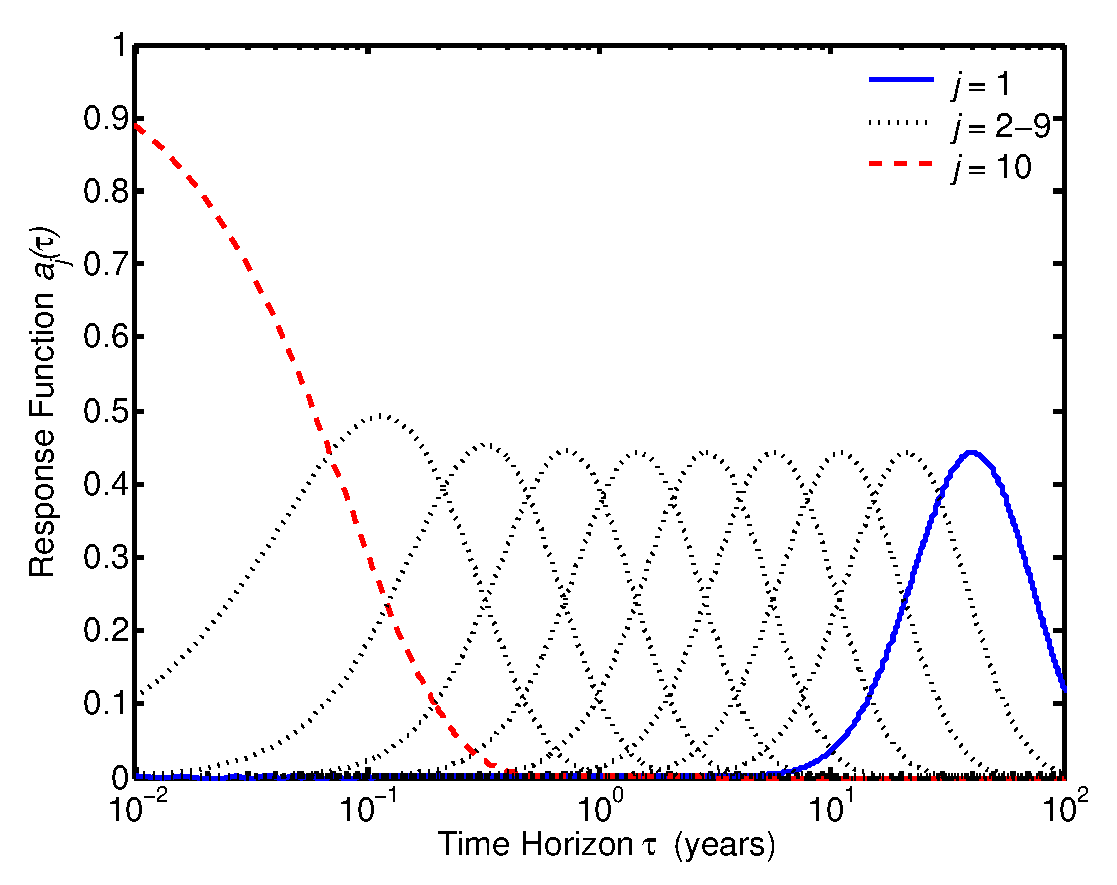
\includegraphics[height=4.0in,width=6in]{figlxffloading_numexmp.eps}
\end{center}
  \caption{The instantaneous interest rate response to unit shocks from different frequency components.}

Lines plot the response of the instantaneous interest rate to unit shocks from
each of the 15 frequency components across different time horizons. The solid
line denotes response to shocks from the lowest frequency $dW_{1,t}$, the
dashed line denotes response to shocks from the highest frequency $dW_{15,t}$.
The dotted lines represent responses to intermediate frequency components. The
responses are computed with the parameters $\kappa_r=1/30$, $b=1.69$, and
$n=15$.
   \label{f:numexmp}
\end{figure}

%*************************Figure 2******************************;
\begin{figure}[e]
\begin{center}
  \includegraphics[height=4in,width=6in]{figliborswapts.eps}
  \includegraphics[height=4in,width=6in]{figliborswapterm.eps}
\end{center}
  \caption{LIBOR and swap time series and term structure.}

The top panel plots the time series of the 15 LIBOR/swap rate series. The
bottom panel plots the term structure at each date.
   \label{f:liborswapts}
\end{figure}

%Reduce the clustering in the plot: Three-4 lines in each graph.


%*************************Figure 3******************************;
\begin{figure}[e]
\begin{center}
\begin{tabular*}{\hsize}{c}
Piece-wise constant forward curves\\
 \includegraphics[height=4in,width=6in]{figforwardsFL.eps}
  \\
 Model-generated forward curves \\
  \includegraphics[height=4in,width=6in]{figforwardscascade02cr6.eps}
  \end{tabular*}
  \end{center}
  \caption{Term structure of forward rates stripped from LIBOR and swap rates}

Lines plot the term structure of forward rates generated from the piece-wise constant assumption in the top panel and from the estimated
15-factor model in
the bottom panel.
   \label{f:spot}
\end{figure}


%*************************Figure 4******************************;

\begin{figure}[e]
\begin{center}
  \includegraphics[height=4in,width=6in]{figcorrratesM6m.eps}
\end{center}
  \caption{Cross-correlation between weekly changes in six-month LIBOR and other interest rate series.}

Circles denote the cross-correlation estimates between weekly changes in the
six-month LIBOR and weekly changes in other interest rate series. The solid
line denotes estimates from model values generated from the 15-factor model.
The dashed line denotes estimates from model values generated from the
three-factor model.
   \label{f:corr}
\end{figure}

%In-sample vs. population: how different are they in our model?

%*************************Figure 5******************************;

\begin{figure}[e]
\begin{center}
%  \includegraphics[height=2.0in,width=3.15in]{figkappav_cascade02p2.eps}
  \includegraphics[height=4in,width=6in]{figlnkappav_cascade02p2.eps}
\end{center}
  \caption{The scaling of $\kappa_j$.}
  The circles are estimated as free parameters. The solid line is generated from the benchmark model with the scaling $\kappa_i=\kappa_1 b^{i-1}$.

   \label{f:kappaj}
\end{figure}




\end{document}
